\chapter{Reminders}

I first start by  reminders of classical mechanics, probabilities and standard quantum mechanics. 
This is mostly very standard material, taken from notes of my graduate courses (Master level) in Quantum Field Theory.
The sections on classical and quantum probabilities are a bit more original.



\section{Classical mechanics}
\index{Classical mechanics}
The standard books on classical mechanics are the books by Landau \& Lifshitz \cite{LandauMechanics76} and the book by A. Arnold \cite{ArnoldMechanics89}.

\subsection{ Lagrangian formulation}
\index{Lagrangian}
Consider the simplest system: a non relativistic particle of mass $m$ in a one dimensional space (a line). 
Its coordinate (position) is denoted $q$. It is submitted to a conservative force which derives from a potential $V(q)$. 
The potential is independent of time.
The velocity is $\dot{q}(t)={dq\over dt}$.
The dynamics of the particle is given by Newton's equation
\index{Newton's equation}
\begin{equation}
\label{neweq}
m\,\ddot{q}(t)=-{\partial\over\partial q}\, V(q)
\end{equation}
The equation of motion derives from the least action principle. The classical trajectories extremize the action $S$
\index{Action}
\begin{equation}
\label{actlagr}
S[q]=\int_{t_i}^{t_f} dt\ L(q(t),\dot{q}(t))
\qquad,\qquad
L(q,\dot{q})={m\over 2}\dot{q}^2-V(q)
\end{equation}
$L$ is the lagrangian. 
\index{Lagrangian}
Under the variations  the initial and final positions are fixed $q(t_i)=q_i$, $q(t_f)=q_f$. So one requires that a classical solution $q_c(t)$ satisfies
\begin{equation}
\label{varact0}
q(t)=q_c(t)+\delta q(t)\ ,\quad \delta q(t_i)=\delta q(t_f)=0\quad\implies\quad
S[q]=S[q_c]+\mathcal{O}(\delta q^2)
\end{equation}
This functional derivative equation leads to the Euler-Lagrange equation \index{Euler-Lagrange equation}
\begin{equation}
\label{vareq1}
{\delta S[q]\over\delta q(t)}=0
\qquad\iff\qquad
{d\over dt}\,{\partial L(q,\dot{q})\over\partial \dot{q}(t)}={\partial L(q,\dot{q})\over\partial {q}(t)}
\end{equation}
which leads to \ref{neweq} 
\begin{figure}[h]
\begin{center}
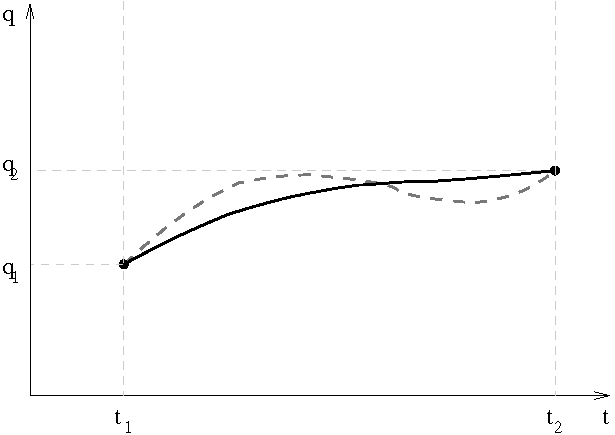
\includegraphics[width=3in]{VarPrincLagrange.pdf}
\caption{The least action principle: the classical trajectoire (full line)  extremizes the action. Under a variation (dashed line) $\delta S=0$. The initial and final positions are kept fixed.}
\label{ }
\end{center}
\end{figure}
This generalizes to many systems: higher dimensional space, many particles, systems with internal degrees of freedom, time-dependent potentials, fields, as long as there is no irreversibility (dissipation).

A good understanding of the origin of the least action principle in classical mechanics comes in fact from the path integral formulation of quantum mechanics.


\subsection{Hamiltonian formulation}
\subsubsection{Phase space and Hamiltonian:} 
\index{Phase space}
\index{Hamiltonian}
The Hamiltonian formulation is in general equivalent, but slightly more general than the Lagrangian formulation.
For a classical system with $n$ degrees of freedom, a state of a system is a point $\boldsymbol{x}$ in the phase space 
$\boldsymbol{\Omega}$ of the system. $\boldsymbol{\Omega}$ is a manifold with even dimension $2n$. 
The evolution equations are flow equations (first order differential equations in time) in the pause space.


For the particle in dimension $d=1$ in a potential there is one degree of freedom, $n=1$ and dim($\Omega$)=2.
The two coordinates  in phase space are the  position $q$ et the momentum $p$.

\begin{equation}
\label{ }
\mathbf{x}=(q,p)
\end{equation}
The Hamiltonian is
\begin{equation}
\label{hamilt1}
H(q,p)={p^2\over 2m}+V(q)
\end{equation}
The equations of motion are the  Hamilton equations
\index{Hamilton equations}
\begin{equation}
\label{hamilt2}
\dot{p}=-{\partial H\over\partial q}
\qquad,\qquad
\dot{q}={\partial H\over\partial p}
\end{equation}
so the relation between the momentum and the velocity $p=m\dot q$ is a dynamical relation.
The Hamilton equations derive also from a variational principle. To find the classical trajectory such that 
$q(t_1)=q_1$, $q(t_2)=q_2$
one extremizes the action functional 
  $\mathcal{S}_H$
\begin{equation}
\label{hamilt3b}
\mathcal{S}_H [q,p]=\int_{t_1}^{t_2} dt\,\left[{p(t)\dot{q}(t)-H(q(t),p(t))}\right]
\end{equation}
with respect to variations of 
$q(t)$ and of  $p(t)$, $q(t)$ being fixed at the initial and final times $t=t_1$ et $t_2$, but $p(t)$ being free at  $t=t_1$ and $t_2$.
Indeed, the functional derivatives of $\mathcal{S}_H$ are
\begin{equation}
\label{hamilt3}
{\delta \mathcal{S}_H \over\delta q(t)}=-\dot p(t)-{\partial H\over\partial q}(q(t),p(t))
\ ,\quad
{\delta \mathcal{S}_H \over\delta p(t)}=\dot q(t)-{\partial H\over\partial p}(q(t),p(t))
\end{equation}
The change of variables $(q,\dot q)\to(q,p)$ and of action  fonctionals  $S(q,\dot q)\to \mathcal{S}_H (q,p)$ between the Lagrangian and the Hamiltonian formalism corresponds to a  Legendre transform.
\begin{figure}[h]
\begin{center}
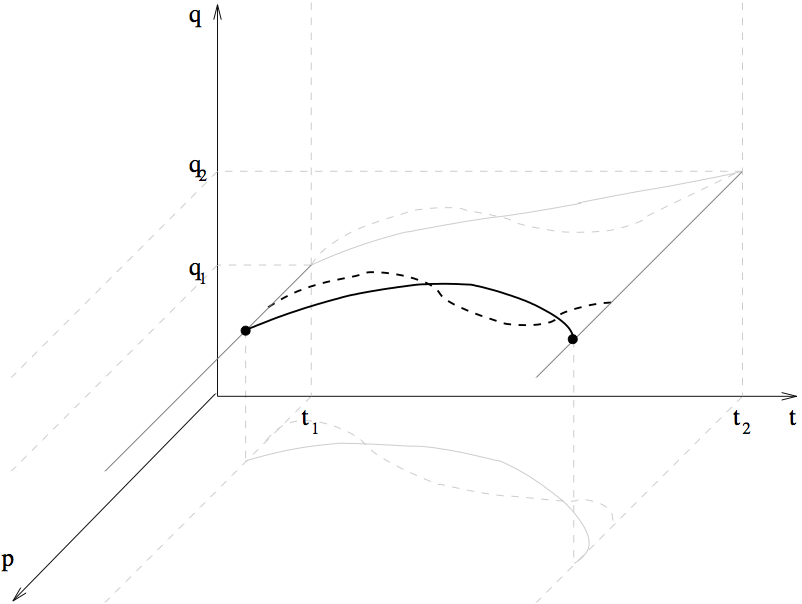
\includegraphics[width=3in]{VarPrincHamilton.png}
\caption{Least action principle in phase space: The classical trajectory (full line) extremizes the action $S_H[q,p]$.
The initial and final positions are fixed. The initial and final momenta are free. Their actual value is given by the variational principle as a function of the initial and final positions and times.}
\label{ }
\end{center}
\end{figure}


\subsubsection{Hamilton-Jacobi equation} 

For a classical trajectory $q_\mathrm{cl}(t)$ solution of the equations of motion, the action functionals $\mathcal{S}_H$ and $S$ are equal!
If we fix the initial time $t_1$ and the initial position $q_1$, this classical action can be considered as a function of the final time $t_2={t}$ and of the final position $q(t_2)=q_2={q}$. This function is called the Hamilton-Jacobi action, or the Hamilton function, and I note it $\mathcal{S}(q,t)=\mathcal{S}_{\scriptscriptstyle{\mathrm{HJ}}}({q},{t})$ to be explicit (the initial conditions $q(t_1)=q_1$ being implicit)
\index{Hamilton-Jacobi action}
\begin{align}
\label{ }
\mathcal{S}(q,t)=\mathcal{S}_{\scriptscriptstyle{\mathrm{HJ}}}({q},{t})=
\mathcal{S}[q_{\mathrm{cl}}] \quad&\text{with}\ q_{\mathrm{cl}}\ \text{classical solution such that}\quad {q(t_2)={q}, t_2={t}}\ 
\nonumber\\
&\text{and where}\ t_1\ \text{and}\ {q(t_1)=q_1}\ \text{are kept fixed}
\end{align}

Using the equations of motion it is easy to see that the evolution with the final time $t$ of this function $\mathcal{S(}q,t)$ is given by the differential equation
\index{Hamilton-Jacobi Equation}
\begin{equation}
\label{ }
{\partial\mathcal{S}\over\partial t}=-H\left(q,{\partial\mathcal{S}\over\partial q}\right)
\end{equation}
with $H$ the Hamiltonian function.
This is is a first order differential equation with respect to the final time $t$. It is called the Hamilton-Jacobi equation.

From this equation on can show that (the initial conditions $(t_1,q_1)$ being fixed) the impulsion $p$ and the total energy $E$ of the particle at the final time $t$, expressed as a function of its final position $q$ and of $t$, are 
\begin{equation}
\label{ }
E(q,t)=-{\partial\mathcal{S}\over\partial t}(q,t)\ ,\quad p(q,t)={\partial\mathcal{S}\over\partial q}(q,t)
\end{equation}
These formulas extends to the case of systems with $n$ degrees of freedom and of mote gerenal Hamiltonians.
Positions and momenta are now $n$ components vectors
\begin{equation}
\label{ }
\mathbf{q}=\{q^i\}\quad,\qquad \mathbf{p}=\{p_i\}\qquad i=1,\cdots,n
\end{equation}


\subsubsection{Symplectic manifolds} 

\index{Symplectic manifold} 
\index{Phase space} 


A more general situation is a general system whose phase space $\mathbf{\Omega}$ is a manifold with an even dimension $N=2n$,  not necessarily the Euclidean space $\mathbb{R}^{N}$, but with for instance a non trivial topology.
Locally $\mathbf{\Omega}$ is described by local coordinates $\mathbf{x}=\{x^i,i=1,2n\}$ (warning! The $x-i$ are coordinate in phase space, not some position coordinates in physical space).

Hamiltonian dynamics requires a symplectic structure on $\Omega$. This symplectic structure allows to define (or amounts to define) the Poisson brackets. $\Omega$ is a symplectic manifold if it is embodied with an antisymmetric 2-form  $\omega$ (a degree 2 differential form) which is non-degenerate and closed ($d\omega=0$).
This means that to each point  $\mathbf{x}\in\Omega$ is associated (in the coordinate system $\{x�\}$
$$\omega(\mathbf{x})={1\over 2}\omega_{ij}(\mathbf{x}) dx^i \wedge dx^j$$
caracterized by an antisymmetric matrix  $2n\times 2n$ which is invertible
$$w_{ij}(\mathbf{x})=-w_{ji}(\mathbf{x})\quad,\qquad \det(\omega)\neq 0$$
$dx^i\wedge dx^j$ is the antisymmetric product (exterior product) of the two 1-forms $dx^i$ and $dx^j$.
This  form is closed. Its exterior derivative $d\omega$ is zero
$$ d\omega(\mathbf{x})={1\over 3!}\sum_{i,j,k} \partial_i \omega_{jk}(\mathbf{x})\, dx^i\wedge dx^j\wedge dx^k = 0$$
In term of components this means
 $$\forall\  i_1<i_2<i_3\quad,\qquad \partial_{i_1}\omega_{i_2 i_3}+\partial_{i_2}\omega_{i_3 i_1}+\partial_{i_3}\omega_{i_1 i_2}=0$$
The fact that $\omega$ is a differential form means that under a local change of coordinates $\mathbf{x}\to\mathbf{x'}$ (in phase space) the components of the form change as
 $$\mathbf{x}\to\mathbf{x'}\quad,\qquad  \omega=\omega(\mathbf{x})_{ij}\,dx^i\wedge dx^j=\omega'(\mathbf{x}')_{ij}\,d{x'}^i\wedge d{x'}^j$$
that is for the components
 $$  \omega'(\mathbf{x}')_{ij} =  \omega(\mathbf{x})_{kl}\ {\partial  x^k\over \partial {x'}^i} {\partial  x^l\over \partial {x'}^j} $$
The Poisson brackets will be defined in the next subsection.%

For the particule on a ligne $n=1$, $\mathbf{\Omega}=\mathbb{R}^2$, $\mathbf{x}=(q,p)$,
The symplectic form is simply $\omega= dq\wedge dp$. Its components are
\begin{equation}
\label{omegan1}
\omega=(\omega_{ij})=\begin{pmatrix}
    0  &  1  \\
    -1  &  0
\end{pmatrix}
\end{equation}
In $d=n$ dimensions $\mathbf{\Omega}=\mathbb{R}^{2n}$, $\mathbf{x}=(q^i,p^i)$, and $\omega={1\over 2}\sum\limits_i dq^i\wedge dp^i$, i.e.
\begin{equation}
\label{omegaDarb}
( \omega_{ij})=\begin{pmatrix}
   0   &   1 & 0 & 0 & \cdots \\
   -1   &  0 & 0 & 0 & \cdots \\
   0 & 0 & 0 & 1 & \cdots \\
   0 & 0 & -1 & 0 & \cdots \\
   \vdots & \vdots & \vdots & \vdots & \ddots
\end{pmatrix}
\end{equation}

The Darboux theorem 
\index{Darboux theorem}
\index{Darboux coordinates}
shows that for any symplectic manifold $\Omega$ with a symplectic form $\omega$, it is always possible to find local coordinate systems (in the neighborhood of any point) such that the symplectic form takes the form \ref{omegaDarb} ($\omega$ is constant and is a direct sum of antisymmetric symbols). The $(q^i,p^j)$ are local pairs of conjugate variables.

The fact that locally the symplectic form may be written under its generic  constant form means that symplectic geometry is characterized only by global invariants, not by local ones. This is different from Riemaniann geometry, where the metric tensor $g_{ij}$ cannot in general be written in its flat form $h_{ij}=\delta_{ij}$, because of curvature, and where there are local invariants.

 \subsubsection{Observables, Poisson brackets}

\index{Observable}
The observables of the system defined by a symplectic phase espace $\Omega$ may be identified with the (``sufficiently regular'') real functions on $\Omega$. The value of an observable $f$ for the system in the state $x$ is simply $f(\mathbf{x})$.
Of course observables may depend explicitly on the time $t$ in addition on $x$.
\begin{equation}
\label{ }
\text{system in state}\ x\quad\to\quad \text{measured value of}\ f\ =\ f(x)
\end{equation}
For two differentiable functions (observables) $f$ and $g$, the Poisson bracket $\{f,g\}_\omega$ is the function (observable) defined by
\index{Poisson bracket}
\begin{equation}
\label{hamilt4}
{\{f,g\}}_\omega(x)=\omega^{ij}(x)\ \partial_i f(x)\,\partial_j g(x)
\quad\text{with}\quad \partial_i={\partial\over\partial x^i}\quad\text{and}\quad w^{ij}(x)=\left(w^{-1}(x)\right)_{ij}
\end{equation}
the matrix elements of the inverse of the antisymmetric matrix $\omega(x)$.
When no ambiguity are present, I shall omit the subscript $\omega$.
In a canonical local coordinate system (Darboux coordinates) the Poisson bracket is
\begin{equation}
\{f,g\}=\sum_i\ {\partial f \over \partial q^i}{\partial g \over \partial p^i}-{\partial f \over \partial p^i }{\partial g \over \partial q^i}
\qquad\hbox{and}\qquad
\{q^i,p^j\}=\delta_{ij}
\end{equation}
The Poisson bracket is  antisymmetric
\begin{equation}
\label{antisymBr}
\{f,g\}=-\{g,f\}
\end{equation}
The fact that it involves first order derivatives only implies the Leibnitz rule (the Poisson bracket acts as a derivation)
\begin{equation}
\label{LeibnitzBra}
\{f,gh\}\ =\ \{f,g\}h+g \{f,h\}
\end{equation}
The fact that the symplectic form is closed $d\omega=0$ is equivalent to the Jacobi identity
\index{Jacobi identity}
\begin{equation}
\label{JacobiBra}
\{f,\{g,h\}\}+\{g,\{h,f\}\}+\{h,\{f,g\}\}=0
\end{equation}
Knowing the Poisson bracket $\{\ ,\}$ is equivalent to know the symplectic form $\omega$ since
\begin{equation}
\label{ }
\{x^i,x^j\}=\omega^{ij}(\mathbf{x})
\end{equation}

\subsubsection{Dynamics, Hamiltonian flows:}
\index{Hamiltonian flow}
In Hamiltonian mechanics, the dynamics of the system is generated by an Hamiltonian function $H$. The Hamiltonian is a real regular (in general differentiable) function on the phase space $\Omega\to\mathbb{R}$.
The state of the system $\mathbf{x}(t)$ changes with time and the evolution equation for the coordinates $x^i(t)$ in phase space  (the Hamilton �quation) take the general form (for a time in dependent Hamiltonian)
\begin{equation}
\label{evolX}
\dot x^i(t)={dx^i(t)\over dt}={\{x^i(t),H\}}
=w^{ij}(\mathbf{x}(t))\,\partial_jH(\mathbf{x}(t))
\end{equation}
This form involves the Poisson Bracket and is covariant under local changes of coordinates in phase espace.
The equations are flow equations of the general form
\begin{equation}
\label{ }
\dot x^i(t)={dx^i(t)\over dt}=F^i(\mathbf{x}(t))
\end{equation}
but the vector field $F^i=\omega^{ij}\partial_jH$ is special and derives from $H$. The flow, i.e. the application
$\phi$: $\Omega\times\mathbb{R}\to \Omega$ is called the Hamiltonian flow associated to $H$.
The evolution functions $\Phi_t(\mathbf{x}$ defined by
\begin{equation}
\label{ }
\mathbf{x}(t=0)=\mathbf{x}\quad\implies\quad \phi_t(\mathbf{x})=\mathbf{x}(t)
\end{equation} 
form a group of transformations (as long as $H$ is independent of the time)
\begin{equation}
\label{ }
\phi_{t_1+t_2}=\phi_{t_1}\circ\phi_{t_2}
\end{equation}
More generally, let us consider a (time independent) observable $f$ (a function on $\Omega$). The evolution of the value of $f$ for a dynamical state $\mathbf{x}(t)$, $f(\mathbf{x},t)=f(\mathbf{x}(t))$ where $\mathbf{x}(t)=\phi_t(\mathbf{x})$, obeys the equation
\begin{equation}
\label{dFdt1}
{\partial f(\mathbf{x},t)\over\partial t}={d f(\mathbf{x}(t))\over dt}={\{f,H\}}(\mathbf{x}(t))
\end{equation}
where the r.h.s. is the Poisson bracket of the observable $f$ and the Hamiltonian $H$.
In particular (when $H$ is independent of $t$) the energy $E(t)=H(\mathbf{x}(t))$ is conserved
\begin{equation}
\label{ }
{\partial E(\mathbf{x},t)\over\partial t}={d H(\mathbf{x}(t))\over dt}=0
\end{equation}


\subsubsection{The Liouville measure}
\index{Liouville measure}
The symplectic form $\omega$ defines an invariant volume element $d\mu$ on the phase space $\Omega$. 
%La mesure de Liouville d�finit l'�l�ment de volume dans l'espace des phases
\begin{equation}
\label{ }
d\mu(\mathbf{x})=\omega^n = \prod_{i=1}^{2 n} d x^i\, | \omega | ^{1/2}
\quad,\qquad  | \omega |=|\det(\omega_{ij})|
\end{equation}
This defines the so-called Liouville measure on $\Omega$. 
This mesure is invariant under all the Hamitonian flows.
% Elle est invariante sous les flots Hamiltoniens, donc sous le transformations canoniques (voir plus loin).

\subsubsection{Example: the classical spin}
\index{Spin}
\index{Classical spin}
The simplest example of a system with a non trivial phase space is the classical spin (the classical top with constant total angular momentum).
The states of the spin are labelled by unit 3-components vector $\vec n=(n_1,n_2,n_3)$, $|\vec n|=1$ (the direction of the angular momentum). Thus the phase space is the 2-dimensional unit sphere and is compact
$$\Omega=\mathcal{S}_2$$
The classical precession equation
$${d\vec n\over dt}=\vec B\times \vec n $$
can be written in Hamiltonian form.
$\vec B$ is a vector in $\mathbb{R}^3$, possibly a 3-component vector field on the sphere depending on $\vec n$. 

There is a symplectic structure on $\Omega$. It is related to the natural complex structure on $\mathcal{S}_2$ (the Riemann sphere).
The Poisson bracket of two functions $f$ and $g$ on $\mathcal{S}_2$ is defined as
$$\{f,g\}=(\vec \nabla f \times \vec\nabla g )\cdot \vec n\ .$$
The gradient field $\vec\nabla f$ of a function $f$ on the sphere is a vector field  tangent to the sphere, so $\vec \nabla f \times \vec\nabla g$ is normal to the sphere, hence collinear with $\vec n$.
In spherical coordinates
$$  \vec n=(\sin\theta \cos\phi,\sin\theta \sin\phi, \cos\theta) $$
the Poisson bracket is simply
$$
\{f,g\}={1\over\sin\theta}\left({\partial f\over\partial\theta}{\partial g\over\partial\phi}-  {\partial g\over\partial\theta}{\partial f\over\partial\phi}\right)
$$
Admissible local Darboux coordinates $\mathbf{x}=(x^1,x^2)$ such that $\omega= dx^1\wedge dx^2$ must be locally orthogonal, area preserving mappings. 
\index{Darboux coordinates}
Examples are 
\begin{itemize}
  \item  
``action-angle'' variables (the Lambert cylindrical equal-area projection)
$$\mathbf{x}=(\cos\theta,\phi)$$
 \item or plane coordinates (the Lambert azimuthal equal-area projection).
$$\mathbf{x}=(2\sin(\theta/2)\cos\phi,2\sin(\theta/2)\sin\phi)$$
\end{itemize}
\index{Lambert coordinates}
\begin{figure}[h]
\begin{center}

\includegraphics[height=1.2in]{Lambert_cylindrical_equal-area_projection_SW_lt.jpg}
\qquad

\includegraphics[height=2.in]{Lambert_azimuthal_equal-area_projection_SW_lt.jpg}
\medskip
\caption{The Lambert cylindrical and azimuthal coordinates}
\label{ }
\end{center}
\end{figure}
%
With this Poisson bracket, the Hamiltonian which generates the precession dynamics is simply (for constant $\vec B$)
$$H=\vec B\cdot\vec n$$

\subsubsection{Statistical states, distribution functions, the Liouville equation}
\index{Statistical ensemble}
\index{Statistical distribution}
\index{Mixed state}
\index{Expectation value}
We now consider statistical ensembles. If we have only some partial information on the state of the system, to this information is  associated  a statistical (or mixed) state $\varphi$. This statistical state is described by a probability distribution on the phase space $\Omega$, that we write
\begin{equation}
\label{ }
d\rho_\varphi(\mathbf{x})=d\mu(\mathbf{x})\, \rho_\varphi(\mathbf{x})
\end{equation}
with $d\mu(\mathbf{x})$ the Liouville measure and $\rho_\varphi(\mathbf{x})$ the probability density, a non negative distribution (function) such that
\begin{equation}
\label{ }
\rho_\varphi(\mathbf{x})\ge 0\quad,\qquad \int_\Omega d\mu(\mathbf{x})\, \rho_\varphi(\mathbf{x})=1
\end{equation}
On a given statistical state $\varphi$ the expectation for an observable $f$ (its expectation value, i.e. its mean value if we perform a large number of measurements of $f$ on independent systems in the same state $\varphi$) is 
\begin{equation}
\label{ }
\langle f\rangle_\varphi = \int_\mathbf{\Omega} d\mu(\mathbf{x})\, \rho_\varphi(\mathbf{x})\, f(\mathbf{x})
\end{equation}

When the system evolves according to some Hamiltonian flow $\phi_t$ generated by a Hamiltonian $H$, the statistical state depends on time 
$\varphi\to \varphi(t)$, as well as the distribution function $\rho_\varphi\to\rho_{\varphi(t)}$. 
$\varphi$ being the initial state of the system at time $t=0$, we can denote this function
\begin{equation}
\label{ }
\rho_{\varphi(t)}(\mathbf{x})=\rho_\varphi(\mathbf{x},t)
\end{equation}
This time dependent distribution function is given by
\begin{equation}
\label{ }
\rho_\varphi(\mathbf{x}(t),t)=\rho_\varphi(\mathbf{x}) \quad,\qquad \mathbf{x}(t)=\phi_t(\mathbf{x})
\end{equation}
(using the fact that the Liouville measure is conserved by the Hamiltonian flow).
Using the evolution equation for $\mathbf{x}(t)$  \ref{evolX}, one obtains the evolution equation for the distribution function $\rho_\varphi(\mathbf{x},t)$, called the Liouville equation 
\index{Liouville equation}
\begin{equation}
\label{LiouvilleEq}
{\partial\over \partial t}\rho_\varphi(\mathbf{x},t)=\left\{H,\rho_\varphi\right\}(\mathbf{x},t)
\end{equation}
$\left\{H,\rho_\varphi\right\}$ is the Poisson bracket of the Hamiltonian $H$ and of the density function $\rho_\varphi$, considered of course as a function of $\mathbf{x}$ only (time is fixed in the r.h.s. of \ref{LiouvilleEq}).

With these notations, the expectation of the observable $f$ d�pends on the time $t$ , and is given by the two equivalent integrals
\begin{equation}
\label{ }
\langle f\rangle(t)=\int_\mathbf{\Omega} d\mu(\mathbf{x})\, \rho_\varphi(\mathbf{x})\, f(\mathbf{x}(t))= \int_\mathbf{\Omega} d\mu(\mathbf{x})\, \rho_\varphi(\mathbf{x},t)\, f(\mathbf{x})
\end{equation}

Of course when the state of the system is a ``pure state'' ($\varphi_\mathrm{pure}=\mathbf{x}_0$) the distribution function is a Dirac measure $\rho_\mathrm{pure}(\mathbf{x})=\delta(\mathbf{x}-\mathbf{x}_0)$ and the Liouville equation leads to
\begin{equation}
\label{ }
\rho_\mathrm{pure}(\mathbf{x},t)=\delta(\mathbf{x}-\mathbf{x}(t))
\quad,\qquad \mathbf{x}(t)=\phi_t(\mathbf{x}_0)
\end{equation}
\index{Pure state}


\subsubsection{Canonical transformations}
\index{Canonical transformation}
The Hamiltonian flow is an example of canonical transformations.
Canonical transformations $\mathcal{C}$ are (bijective) mappings $\mathbf{\Omega}\to\mathbf{\Omega}$ which preserve the symplectic structure.
Denoting the image of the point $\mathbf{x}\in\Omega$ (by the canonical transformation $\mathcal{C}$) by $\mathbf{X}$
\begin{equation}
\label{defmapC}
\mathbf{x}\  \mathop{\to}^\mathcal{C}\ \mathbf{X}=\mathcal{C}(\mathbf{x})
\end{equation}
This means simply that the symplectic form $\omega^*$ defined by
\begin{equation}
\label{omegastar}
\omega^*(x)=\omega(X)
\end{equation}
is equal to the original form
\begin{equation}
\label{ }
\omega^*=\omega
\end{equation}
$\omega^*$ is called the pullback of the symplectic form $\omega$ by the mapping $\mathcal{C}$ and is also denoted $\mathcal{C}^*\omega$.
In a given coordinate system such that
\begin{equation}
\label{ }
\mathbf{x}=(x^i)\ ,\ \ 
\mathbf{X}=(X^k)
\end{equation}
\ref{omegastar} means that $\omega$ and $\omega^*$ read
\begin{equation}
\label{ }
\omega(x)=w_{ij}(\mathbf{x})\,dx^i\wedge dx^j 
\quad,\qquad
\omega^*(x)=w_{ij}(\mathbf{X})\,dX^i\wedge dX^j 
\end{equation}
so that the components of $\omega^*$  are
\begin{equation}
\label{ }
\omega^*_{ij}(\mathbf{x})=w_{kl}(\mathbf{X})  {\partial X^k\over\partial x^i}{\partial X^l\over\partial x^j}
\end{equation}
$\mathcal{C}$ is a canonical transformation if
\begin{equation}
\label{ }
\omega_{ij}(\mathbf{x})=\omega^*_{ij}(\mathbf{x})
\end{equation}

Canonical transformations are the transformations that preserve the Poisson brackets. Let $f$ and $g$ be two observables (functions $\Omega\to\mathbb{R}$ and $F=f\circ \mathcal{C}^{-1}$ and $G=g\circ \mathcal{C}^{-1}$ their transform by the transformation $\mathcal{C}$
\begin{equation}
\label{ }
f(\mathbf{x})=F(\mathbf{X})\quad,\qquad g(\mathbf{x})=G(\mathbf{X})
\end{equation}
$\mathcal{C}$ is a canonical transformation if
\begin{equation}
\label{ }
\{f,g\}_\omega=\{F,G\}_\omega
\end{equation}
Taking for $f$ and $g$ the coordinate change $x^i\to X^i$ itself, canonical transformations are change of coordinates such that
\begin{equation}
\label{ }
\{X^i,X^j\}=\{x^i,x^j\}
\end{equation}

Canonical transformations are very useful tools in classical mechanics. They are the classical analog of unitary transformations in quantum mechanics.

In the simple example of the classical spin, the canonical transformations are simply the smooth area preserving diffeomorphisms of the 2 dimensional sphere.


\subsubsection{Along the Hamiltonian flow}

As an application, one can treat the Hamiltonian flow $\phi_t$ as a time dependent change of coordinate in phase space (a change of reference frame) and look at the dynamics of the system in this new frame which moves with the system.
In this new coordinates, denoted $\bar{\mathbf{x}}=\{\bar x^i\}$, if at time $t=0$ the system is in an initial  state $\bar{\mathbf{x}}=\mathbf{x}_0$, at time $t$ it is of course still in the same state
$\bar{\mathbf{x}}(t)=\mathbf{x}_0$.
\index{Hamiltonian flow}

It is the observables $f$ which become time dependent.
Indeed, if in the original (time independent) coordinate system one considers a time independent observable $f$ (a function $\mathbf{x}\to f(\mathbf{x})$), in the new coordinate system one must consider the time dependent observable $\bar f$, defined by
\begin{equation}
\label{ }
\bar f(\mathbf{\bar x}, t)=f(\mathbf{x}(t))
\qquad\text{with}\quad \mathbf{x}(t)=\phi_t(\mathbf{\bar x})\quad\text{i.e.}\quad \mathbf{x}(0)=\mathbf{\bar x}
\end{equation}
This time dependent observable $\bar f(\mathbf{\bar x},t)$ describes how the value of the observable $f$ evolves with the time $t$, when expressed as a function of the initial state $\mathbf{\bar x}$.
Of course the time  evolution of $\bar f$ depends on the dynamocs of the system, hence of the Hamiltonian $H$.
The dynamics for the observables is given by evolution equation (similar to the Liouville equation, up to a sign)
\begin{equation}
\label{LEqF}
{\partial\bar f\over \partial t}=- \{H,\bar f\}
\quad\text{i.e.}\qquad
{\partial\bar  f(\mathbf{\bar x},t)\over \partial t}=\{\bar f,H\}(\mathbf{\bar x},t)
\end{equation}
In this dynamical frame the Hamiltonian is still time independent, i.e. $\bar H=H$, since its evolution equation is
\begin{equation}
\label{ }
{\partial H \over \partial t}=- \{H,H\}=0
\end{equation}
The Poisson bracket is always the Poisson bracket for the symplectic form $\omega$, since $\omega$ is conserved by the canonical transformations, in particular this change of reference frame.

This change of frame corresponds to a change from a representation of the dynamics by a flow of the states in phase space, the observables being fixed functions, to a representation where the states do not move, but where there is a flow for the functions.
This is the analog for Hamiltonian flows to what is done in fluid dynamics: going from the Eulerian specification (the fluid moves in a fixed coordinate system) to the Lagrangian specification (the coordinate system moves along the fluid).
But these two representations are of course the classical analog of the Schr�dinger picture (vector states evolves, operators are fixed) and of the Heisenberg picture (vector states are fixed, operators depend on time) in quantum mechanics.
\index{Lagrangian specification}
\index{Eulerian specification}


\subsection{The commutative algebra of observables}
\index{Observable}
\index{Commutative algebra}
Let us adopt a slightly more abstract point of view. 
The (real or) complex functions on phase space $f$ $\Omega\to\mathbb{C}$ form a commutative algebra $\mathcal{A}$ with the standard addition and multiplication laws.
\begin{equation}
\label{ }
(f+g)(x)=f(x)+g(x)\quad,\qquad (fg)(x)=f(x) g(x)
\end{equation}
This is more generally true if $\Omega=X$ is simply a locally compact topological space, and $\mathcal{A}$ the algebra of continuous functions with compact support. 

Statistical states (probability distributions on $X$) are then normalized positive linear forms $\varphi$ on $\mathcal{A}$
\begin{equation}
\label{ }
\varphi(\alpha f+\beta g)=\alpha \varphi(f) + \beta \varphi(g)
\ ,\quad
\varphi( f f^*)\ge 0
\ ,\quad
\varphi(1)=1
\end{equation}
The sup or $\mathcal{L}^\infty$ norm, defined as
\begin{equation}
\label{ }
\| f\|^2=\sup_{x\in X} |f(x)|^2 =\sup_{\varphi\,\mathrm{states}} \varphi(|f(x)|^2 )
\end{equation}
has clearly the following properties
\begin{equation}
\label{ }
\| f \|=\| f^* \|
\ ,\quad
\| fg\|\le\| f \| \ \| g\|
\ ,\quad
\| f f^* \| =\| f \|^2
\end{equation}
and $\mathcal{A}$ is complete under this norm. This makes the algebra $\mathcal{A}$ a so-called commutative C$^*$-algebra.
\index{C$^*$-algebra}

For any element $x\in X$, consider the subalgebra of the functions that vanish at $x$
\begin{equation}
\label{ }
\mathcal{I}_x:\{f\in\mathcal{A};\ f(x)=0\}
\end{equation}
They are maximal ideals of $\mathcal{A}$, (left-)ideals $\mathcal{I}$ of an algebra $\mathcal{A}$ being subalgebras of $\mathcal{A}$ such that $x\in\mathcal{I}$ and $y\in\mathcal{A}$ implies $xy\in\mathcal{I}$. It is easy to show that the set of maximal ideals of $\mathcal{A}=C(X)$ is isomorphic to $X$, and that $\mathcal{A}/\mathcal{I}_x=\mathbb{C}$ the target space.

Now a famous theorem by Gelfand and Naimark states that the reciprocal is true. Any commutative C$^*$-algebra is isomorphic to the algebra of continuous functions on some topological (locally compact) space $X$! This seems a formal result (the space $X$ and its topology may be quite wild, and very far from a regular smooth manifold), but it is important to keep in mind that a mathematical object (here a topological space) can be defined intrinsically (by its elements) or equivalently by the abstract properties of some set of functions from this object to some other object (here the commutative algebra of observables). This modern point of view in mathematics (basically this idea is at the basis of the category formalism) is also important in modern physics, as we shall see later in the quantum case.
\index{Gelfand-Naimark}

For the Hamiltonian systems, the algebra of (differentiable) functions on $\Omega$ is equipped with a additional product, the Poisson bracket $\{f,g\}$.
The corresponding algebra, with the three laws (addition, multiplication, Poisson bracket) is now a commutative Poisson algebra.
A Poisson algebra is a (not necessarily commutative) associative algebra with a bracket that satisfies \ref{antisymBr}, \ref{LeibnitzBra} and \ref{JacobiBra}.
\index{Poisson algebra}

\subsection{"Axiomatics"}
The most general formulation for classical Hamiltonian dynamics is that of Poisson manifold. This is a more general formulation that symplectic manifolds, since it encompasses special situations where the symplectic form is degenerate.
Poisson manifolds can in general be split (foliated) into ``symplectic leaves'' embodied with a well defined induced symplectic structure.

The fact that in classical mechanics dynamics are given by Hamiltonian flows on a phase space which is a symplectic or Poisson manifold can be somehow justified, if one assumes that the possible dynamics are flows generated by some smooth vector fields, that these flows are generated by conserved quantities (Hamiltonians) and that these dynamics are covariant under change of frames generated by these flows (existence and invariance of canonical transformations). 
\index{Poisson manifold}

However a real understanding and justification of classical Hamiltonian dynamics comes from quantum mechanics.
Indeed, the Poisson bracket structure is the ``classical limit'' of the commutators of observables (operators)  in quantum mechanics, and the canonical transformations are the classical version of unitary transformations.



\section{Probabilities}
\index{Probabilities}

Probabilities are an important aspect of classical physics and are one of the essential components of quantum physics. 
Without going into any details and any formalism, I think it is important to recall the two main ways to consider and use probabilities in statistics and physics: the frequentist point of view and the Bayesian point of view. At the level considered here, these are  different point of views on the same mathematical formalism, and on its use. As we shall see, in some sense quantum mechanics forces us to treat them on the same footing.
There are of course many different, more subtle and more precise mathematical as well as philosophical points of view on probability theory. I shall not enter in any discussion about the merits and the consistency of objective probabilities versus subjective probabilities.

Amongst  many standard references on the mathematical formalism of probability, there is the book by Kolmogorov
\cite{Kolmogorov-book},
and the book by Feller \cite{Feller-book}. 
See also the quick introduction for and by a physicist by M. Bauer (in french) \cite{BauerCours2009}.
References on Bayesian probabilities are the books by de Finetti \cite{deFinetti-book}, by Jaynes \cite{Jaynes-Book} and the article by Cox \cite{Cox1946}.


\subsection{The frequentist point of view}
\index{Frequentist probabilities}
The frequentist point of view is the most familiar and the most used in statistical physics, dynamical systems, as well as in mathematics (it is at the basis of the formulation of modern probability theory from the beginning of 20th century, in particular for the Kolmogorov axiomatic formulation of probabilities). 
Roughly speaking, probabilities represent a measure of ignorance on the state of a system, coming for instance from: uncertainty on its initial state, uncertainty on its dynamical evolution due to uncertainty on the dynamics, or high sensibility to the initial conditions (chaos). 
Then probabilities are asymptotic frequencies of events (measurements) if we repeat observations on systems prepared by the same initial procedure.
More precisely, one has a set $\Omega$ of samples (the sample space), a $\sigma$-algebra  $\mathcal{F}$ of ``measurable'' subsets of the sample space $\Omega$, and a  measure $P$ on $\mathcal{F}$ (equivalently a probability measure $\mu_\mathcal{F}$ on $\Omega$.
This probability measure is a priori given.

\subsection{The Bayesian point of view}
\index{Bayesian probabilities}
The so called Bayesian point of view is somehow broader, and of use in statistics, game theory, economy, but also in experimental sciences. It is also closer to the initial formulations of probabilities (or ``chance'') in the 18th and 19th centuries. It has been reviewed by statisticians like de Finetti or Jaynes (among others) in the 20th century. 

Probabilities are considered as qualitative estimates for the ``plausibility'' of some proposition (it can be the result of some observation), given some ``state of knowledge'' on a system.
The rules that these probabilities must satisfy are constrained by some logical principles (objectivist point of view where the degree of plausibility is constructed by a ``rational agent''), or may correspond  simply to some ``degree of personal belief'' of  propositions (subjectivist point of view).

\subsection{Conditional probabilities}
\index{Conditional probabilities}
\index{Bayes formula}
The basic rules are the same in the different formulations. A most important concept is conditional probabilities $P(A|B)$ (the probability of $A$,  $B$ being given), and the Bayes (or conditional probability) relation 
\begin{equation}
\label{ }
P(A|B)={P(B|A) P(A)\over P(B)}
\end{equation}
where $P(A)$ and $P(B)$ are the initial probabilities for $A$ and $B$ (the prior), and $P(A|B)$ $P(B|A)$ the conditional probabilities. 

\paragraph{Frequentist:} In the frequentist formulation $P(A|B)$ is the frequency of $A$, once we have selected the samples such that $B$ is true. Bayes formula has the simple representation with Venn diagrams in the set of samples

\begin{figure}[h]
\begin{center}
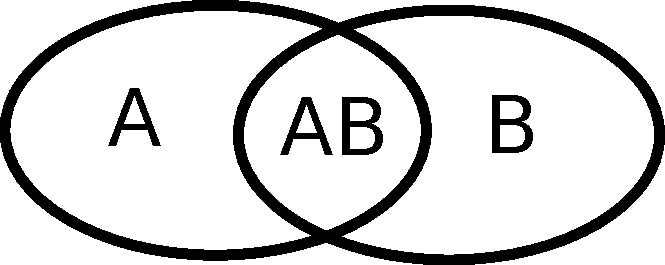
\includegraphics[width=2in]{Venn.pdf}
\caption{Venn representation of the conditional probabilities formula}
\label{ }
\end{center}
\end{figure}

\paragraph{Bayesian:} In the Baysian formulation (see for instance the book by Jaynes), one may consider every probabilities as  conditional probabilities. For instance $P_C(A)=P(A|C)$, where the proposition $C$ corresponds to  the ``prior knowledge'' that leads to the probability assignment $p_C(A)$  for $A$ (so $P_C$ is the probability distribution). If $AB$ means the proposition ``$A$ and  $B$'' ($A\wedge B$ or $A+B$), Bayes formula follows from  the ``product rule''
\begin{equation}
\label{ }
P(AB|C)=P(A|BC) P(B|C)=P(B|AC) P(A|C)
\end{equation}
whose meaning is the following: given $C$, if I already know the plausibility for $AB$ of being true ($P(AB|C)$), and the plausibility for $B$ of being true (the prior $P(B|C)$), the formula tells me how I should modify the plausibility for $A$ of being true, if I learn that $B$ is true ($P(A|BC)$). Together with the ``sum rule''
\begin{equation}
\label{ }
P(A|C)+P(\neg A|C)=1
\end{equation}
($\neg$ is the negation), these are the basic rules of probability theory in this framework.


\section{Quantum mechanics: ``canonical'' formulation}
Let us recall the so called ``canonical formalism'' of quantum mechanics, as it is presented in textbooks. This is the standard presentation when one uses the ``correspondence principle'' to quantize a classical non-relativistic system, or simple field theories.
\index{Canonical quantization}


There is of course an enormous number of good books on quantum mechanics and quantum field theory. 
Among the very first books on quantum mechanics, those  of P. A. Dirac  (1930) \cite{Dirac30} and J. von Neumann (1932) \cite{vonNeumann32G} (\cite{vonNeumann32} for the english traduction of 1955) are still very useful and valuable.
Modern books with a contemporary view and treatment of the recent developments are the books by Cohen-Tanoudji, Laloe \& Diu \cite{Cohen-Tannoudji:1977ys} , by M. le Bellac \cite{LeBellac-2011}, by Auletta, Fortunato and Parisi \cite{Auletta-book-2009}. 

Some standard references on quantum field theory are the books by J. Zinn-Justin \cite{ZinnJustin-book}, by A. Zee \cite{Zee03} (in a very different style). Refernce more oriented towards mathematical physics will be given later.

Amongst the numerous references on the questions of the foundation and the interpretation of quantum mechanics, one may look at the encyclopedic review by Auletta \cite{Auletta}, and at the recent shorter book by F. Laloe \cite{Laloe-book} (see also \cite{Laloe-book-fr,laloe-2001-69}). More later.
\subsection{Principles}

\subsubsection{Pure states:}
\index{Phase space}\index{Hilbert space}
\index{Bra-ket notation}
\index{Scalar product}
\index{Dirac}
The phase space  $\mathbf{\Omega}$ of classical mechanics is replaced by the complex Hilbert space ${\mathcal H}$ of states. 
Elements of $\mathcal{H}$ (vectors) are denoted $\psi$ or $|\psi\rangle$ (``kets'' in Dirac notations). 
The scalar product of two vectors $\psi$ and $\psi'$ in ${\mathcal H}$ is denoted
$\psi^*\!\!\cdot\!\psi'$ or $\langle\psi|\psi'\rangle$. The $\psi^*=\langle\psi\vert$  are the ``bra'' and belong to the dual $\mathcal{H}^*$ of $\mathcal{H}$. 
Note that in the mathematical litterature the scalar product is often noted in the opposite order $\langle\psi\vert\psi'\rangle=\psi'\!\!\cdot\!\psi^*$. We shall stick to the physicists notations.

Pure quantum states are rays of the Hilbert space, i.e. 1 dimensional subspaces of $\mathcal{H}$. They correspond to unit norm vectors $|\psi\rangle$, such that $\|{\psi}\|^2=\langle\psi�|\psi\rangle=1$, and modulo an arbitrary  phase $|\psi\rangle\equiv\emath^{\imath\theta}|\psi\rangle$.



\subsubsection{Observables:} 
\index{Observable}\index{Self-adjoint operator}\index{Physical observable}
The physical observables $A$ are the self-adjoint operators on  $\mathcal{H}$ (Hermitian or symmetric operators), such that $A=A^\dagger$, where the conjugation is defined by $\langle A^\dagger \psi'|\psi\rangle=\langle \psi'|A\psi\rangle$.
Note that the conjugation $A^\dagger$ is rather denoted $A^*$ in the mathematical literature, and in some chapter we shall use this notation, when dealing with general Hilbert spaces not necessarily complex.

The operators on $\mathcal{H}$ form an associative, but non commutative operator algebra.
Any set of of commuting operators $\{A_i\}$ corresponds to a set of classically compatible observables, which can be measured independently.
\index{Non commutative algebra}
\index{Compatible observables}


\subsubsection{Measurements, Born principle:} 
\index{Measurement}
\index{Born principle}
\index{Expectation value}
The outcome of the measurement of an observable $A$ on a state $\psi$ is in general not deterministic. 
Quantum mechanics give only probabilities, and in particular the expectation value of the outcomes. 
This expectation value is given by the Born rule
\begin{equation}
\label{mq1}
\langle A \rangle_{\psi}=\langle\psi|A|\psi\rangle=\langle\psi|A\psi\rangle
\end{equation}
For compatible (commuting) observables the probabilities of outcome obey the standard rule of probabilities and these measurements can be repeated and performed independently.

This implies in particular that the possible outcomes of the measurement of $A$ must belong to the spectrum of $A$, i.e. can only be eigenvalues of $A$ (I consider the simple case where $A$ has a discrete spectrum).
Moreover the probability to get the outcome $a_i$ ($a_i$ being the eigenvalue of $A$ and $|i\rangle$ the corresponding eigenvector) is the modulus squared of the probability amplitude $\langle i|\psi\rangle$
$$  \text{probability of outcome of }A = a_i \text{\ in the state } |\psi\rangle \  =\  p_i\ =\   | \langle i|\psi\rangle |^2$$
\index{Eigenvector}\index{Eigenvalue}\index{Spectrum}

It follows also that quantum measurements are irreversible process. In ideal measurements or non destructive measurements which can be repeated, if the outcome of $A$ was $a_i$, after the measurement the system is found to be in the eigenstate $|i\rangle$. This is the projection postulate.
\index{Irreversible process}
\index{Ideal measurement}
\index{Non-destructive measurement}
\index{Projection postulate}
\index{Orthogonal projector}
In the more general situation where the eigenspace of $A$ associated to the eigenvalue $a_i$ is a higher dimensional subspace $V_i$, the state of the system is obtained by applying the orthogonal projector $P_i$ onto $V_i$ to the initial state $|\psi\rangle$.
Things are more subtle in the case of a continuous spectrum and non normalizable eigenstates.

At that stage I do not discuss what it means to ``prepare a system in a given state'', what ``represents'' the state vector, what is really a measurement process (the problem of quantum measurement) and what means the projection postulate. We shall come back to some of these questions along the course.
\index{Projection postulate}
\index{Measurement}
\index{Preparation}


\subsubsection{Unitary dynamics}
\index{Closed system}
\index{Unitary transformation}
\index{Hamiltonian}
\index{Evolution operator}

For a closed system, the time evolution of the states is linear and it must preserve the probabilities, hence the scalar product $\langle.|.\rangle$. Therefore is given by unitary transformations $U(t)$ such that $U^{-1}=U^\dagger$.
Again if the system is isolated the time evolution form a multiplicative group acting on the Hilbert space and its algebra of observables, hence it is generated by an Hamiltonian self-adjoint operator $H$

$$ U(t)=\exp\left({t\over\imath\hbar}H\right) $$
The evolution equations for states and observables are discussed below.

\subsubsection{Multipartite systems:}
\index{Multipartite system}
\index{Bipartite system}
\index{Tensor product}
\index{Entangled state}
\index{Entanglement}

Assuming that it is possible to perform independent measurements on two independent (causally) subsystems $S_1$ and $S_2$ implies (at least in the  finite dimensional case) that the Hilbert space $\mathcal{H}$ of the states of the composite system $S=``S_1\cup S_2''$ is the tensor product of the Hilbert spaces $\mathcal{H}_1$ and $\mathcal{H}_2$ of the two subsystems.
$$\mathcal{H}=\mathcal{H}_1\otimes \mathcal{H}_2$$
This implies the existence for the system $\mathcal{S}$ of generic ``entangled  states'' between the two subsystems
$$|\Psi\rangle =c { |\psi\rangle}_1\otimes {|\phi\rangle}_2 +  c'  {|\psi'\rangle}_1\otimes {|\phi'\rangle}_2 $$
Entanglement is one of the most important feature of quantum mechanics, and has no counterpart in classical mechanics. 
It is entanglement that leads to many of the counter-intuitive features of quantum mechanics, but  it  leads also to many of its interesting aspects and to some of its greatest success.


\subsubsection{Correspondence principe, canonical quantization}

\index{Canonical quantization}
\index{Correspondence principe}
\index{Conjugate variables}
\index{Commutation relation}
The correspondence principle has been very important in the elaboration of quantum mechanics. Here by correspondence principle I mean that when quantizing a classical system, often one can associate to canonically conjugate variables $(q_i,p_i)$ self-adjoint operators $(Q_i, P_i)$ that satisfy the canonical commutation relations
\begin{equation}
\label{mq2}
\{q_i,p_i\}=\delta_{ij}\ \implies\ [Q_i,P_j]=\imath\hbar\delta_{ij}
\end{equation}
and to take has Hamiltonian the operator obtained by replacing in the classical Hamiltonian the variables $(q_i,p_i)$ by the corresponding operators.
\index{Hamiltonian}
\index{Position}
\index{Momentum}

For instance, for the particle on a line in a potential, one takes as $(Q,P)$ the position and the momentum and for the Hamiltonian
\begin{equation}
\label{HamQV}
H={P^2\over 2m}+V(Q)
\end{equation}
The usual explicit representation is $\mathcal{H}=\mathcal{L}^2(\mathbb{R})$, the states $|\psi\rangle$  correspond to the wave functions $\psi(q)$, and the operators are represented as
\begin{equation}
\label{ }
Q=q\quad,\qquad P={\hbar\over\imath}{\partial\over\partial q}
\end{equation}
\index{Wave function}



\subsection{Representations of quantum mechanics}
The representation of states and observables as vectors and operators is invariant under global unitary transformations (the analog of canonical transformations in classical mechanics). These unitary transformations may depend on time. Therefore there are different representations of the dynamics in quantum mechanics. I recall the two main representations.
La repr�sentation des �tats et des observables �tant invariante par des transformations unitaires globales, pouvant d�pendre du temps (l'�quivalent des transformations canoniques classiques), les �tats et la dynamique du syst�me peuvent se repr�senter de plusieurs fa�on �quivalentes. Je rappelle ici les deux principales.


\subsubsection{The Schr�dinger picture}
\index{Schr�dinger picture}
It is the most simple, and the most used in non relativistic quantum mechanics, in canonical quantization and to formulate the path integral.
In the Schr�dinger picture the states $\psi$ (the kets $|\psi\rangle$) evolve with time and are noted $\psi(t)$. The observables are represented by time independent operators. The evolution is given by the Schr�dinger equation
\index{Schr�dinger equation}\index{State}\index{Observable}
\begin{equation}
\label{mq3}
\imath\hbar{d\psi\over dt}=H\psi
\end{equation}
The expectation value of an observable $A$ measured at time $t$ for a system in the state $\psi$ is thus
\begin{equation}
\label{evAPsi}
\langle A\rangle_{\psi(t)}=
\langle\psi(t)|A|\psi(t)\rangle
\end{equation}
\index{Evolution operator}\index{Evolution equation}
The evolution operator $U(t)$ is defined by 
\begin{equation}
\label{ }
\psi(t=0)=\psi_0\quad \to\quad \psi(t)=U(t)\psi_0
\end{equation}
It is given by
\begin{equation}
\label{ }
U(t)=\exp\left({{t\over\imath\hbar}H}\right)
\end{equation}
and obeys the evolution equation 
\begin{equation}
\label{mq5}
\imath\hbar\,{d \over d t}U(t)=H\ U(t)
\qquad;\qquad
U(0)=\mathbf{1}
\end{equation}
This generalizes easily to the case where the Hamiltonian depends explicitly of the time $t$. Then 
\begin{equation}
\imath\hbar\,{d \over d t}U(t,t_0)=H(t)\ U(t,t_0)
\qquad;\qquad
U(t_0,t_0)=\mathbf{1}
\end{equation}
and
\begin{equation}
\label{mq6b}
U(t,t_0)
=T\left[\exp\left({{1\over\imath\hbar}\int_{t_0}^{t} dt\,H(t)}\right)\right]
=\sum_{k=0}^\infty (\imath\hbar)^{-k}\ \int_{t_0<t_1<\cdots<t_{k}<t} \hskip -4 em dt_1\cdots dt_k\ H(t_{k})\cdots H(t_1)
\end{equation}
where $T$ means the time ordered product (more later).
\index{Time ordered product}


\subsubsection{The Heisenberg picture}
\index{Heisenberg picture}
%\textsl{Raccourcir}
This representation is the most useful in relativistic quantum field theory. It is in fact the best mathematically fully consistent formulation, since the notion of state in more subtle, in particular it depends on the reference frame.
It is required for building the relation between critical systems and Euclidean quantum field theory (statistical field theory).

In the Heisenberg representation, the states are redefined as a function of time via the unitary transformation  $U(-t)$ on $\mathcal{H}$, where $U(t)$ is the evolution operator for the Hamiltonian $H$. They are denoted
 \begin{equation}
\label{mq7}
|\psi;t\rangle=U(-t)|\psi\rangle
\end{equation}
The unitary transformation redefines the observables $A$. They becomes time dependent and are denoted $A(t)$
\begin{equation}
\label{mq9}
A(t)_{}=U(-t)AU(t)
\end{equation}
The dynamics given by the Schr�dinger equation is reabsorbed by the unitary transformation. The dynamical states are independent of time!
\index{Unitary transformation}
\begin{equation}
\label{mq8}
|\psi(t);t\rangle = U(-t)U(t)|\psi\rangle =  |\psi\rangle
\end{equation}
\index{Expectation value}
The expectation value of an observable $A$ on a state $\psi$ at time $t$ is in the Heisenberg representation
\begin{equation}
\label{mq10}
{\langle A(t)\rangle}_{\psi}
=\langle\psi(t);t|A(t)|\psi(t;,t\rangle
=\langle\psi|A(t)|\psi\rangle
\end{equation}
The Schr�dinger and Heisenberg representation are indeed equivalent, since they give the same result for the physical observable (the expectation values)
\begin{equation}
\label{evHevS}
\langle A \rangle_{\psi(t)}={\langle A(t)\rangle}_{\psi}
\end{equation}
\index{Hamiltonian}
In the Heisenberg representation the Hamitonian $H$ remains independent of time (since it commutes with $U(t)$
\begin{equation}
\label{ }
H(t)=H
\end{equation}
The time evolution of the operators is given by the evolution equation
\begin{equation}
\label{mq13}
\imath\hbar{d \over d t}A(t)=[A(t),H]
\end{equation}
\index{Liouville equation}
This is the quantum version of the classical Liouville equation \ref{LEqF}. Of course the Schr�dinger and the Heisenberg representations are the quantum analog of the two ``Eulerian'' and` ``Lagrangian''  representations of classical mechanics discussed above.
\index{Eulerian specification}\index{Lagrangian specification}

For the particle in a potential the equations for $Q$ and $P$ are the quantum version of the classical Hamilton equations of motion
\index{Hamilton equations}
\begin{equation}
\label{mq14}
{d \over d t}Q(t)={1\over m} P(t)
\qquad,\qquad 
{ d\over d t}P(t)=-V'(Q(t))
\end{equation} 
For an observable $A$ which depends explicitly of time (in the Schr�dinger picture), the evolution equation becomes
\begin{equation}
\label{mq13a}
\imath\hbar{d \over d t}A(t)=\imath\hbar{\partial \over \partial t}A(t)+[A(t),H]
\end{equation}
and taking its expectation value in some state $\psi$ one obtains Ehrenfest theorem
\begin{equation}
\label{mq13b}
\imath\hbar{d \over d t}\langle A\rangle (t)=\imath\hbar{\partial \over \partial t}\langle A\rangle (t)+\langle[A,H]\rangle(t)
\end{equation}\index{Ehrenfest's theorem}




\subsection{Quantum statistics and the density matrix}
\index{Quantum statistics}\index{Density matrix}\index{Probabilities}\index{Information}
\subsubsection{The density matrix}
As in classical physics, in general on has only a partial information on the physical system one is interested in.
Its state has to be described by a concept of statistical or mixed state. But in quantum mechanics all the information one can get on a system is provided by the expectation values of the observable of the system. Statistics is already there! The pure quantum states $|\psi\rangle$ are the special ``mixed states'' with the property that a maximal amount of information can be extracted by appropriate sets of compatible measurements on the (ensemble of) state. The difference with classical physics is that different maximal sets of information can be extracted from the same state if one chose to perform different incompatible sets of measurements.

The mathematical concept that represents a mixed state is that of density matrix.
But before discussing this, one can start by noticing that, as in classical physics, an abstract statistical state $\omega$ is fully characterized by the ensemble of the expectation values $\langle A\rangle_\omega$ of all the observables $A$ of the system, measured over the state $\omega$.
\index{Mixed state}\index{Statistical state}\index{Expectation value}\index{Observable}
\begin{equation}
\label{mqst1}
\langle\mathbf{A}\rangle_{\omega}
\quad=\ \text{expectation value of  $\mathbf{A}$ measured over the state $\omega$}
\end{equation}
I denote general statistical states by Greek letters (here $\omega$) and pure states by the bra-ket notation when there is a ambiguity.
The $\omega$ here should not be confused for the notation for the symplectic form over the classical phase space of a classical system. We are dealing with quantum systems and there is no classical phase space anymore.

\index{Operator}\index{Algebra of operator}\index{Linear form}
From the fact that the observables may be represented as an algebra of operators over the Hilbert space $\mathcal{H}$, it is natural to consider that statistical states $\omega$ corresponds to linear forms over the algebra of operators hence applications  $\mathbf{A}\to\langle \mathbf{A}\rangle_\omega$, with the properties
\index{Positivity}
\begin{align}
\label{mqst2}
&\langle a\mathbf{A}+b\mathbf{B}\rangle_\omega=a\langle\mathbf{A}\rangle_\omega+b\langle\mathbf{B}\rangle_\omega
\qquad\text{linearity}\\
&\langle\mathbf{A}^\dagger\rangle_\omega=\overline{\langle\mathbf{A}\rangle}_\omega
\qquad \text{reality}\\
&\langle \mathbf{A}^\dagger \mathbf{A}\rangle_{\omega}\ge 0\qquad 
\text{and}\qquad \langle \mathbf{1}\rangle_{\omega}=1
\qquad\text{positivity and normalization}
\end{align}
For finite dimensional Hilbert spaces and for the most common infinite dimensional cases (for physicists) this is equivalent to state that to any statistical state is associated a normalized positive self-adjoint matrix $\rho_\omega$ such that
\begin{equation}
\label{mqst3}
\langle \mathbf{A}\rangle_{\omega}=\tr (\rho_\omega\, \mathbf{A})
\end{equation}
This is the density matrix or density operator. It was introduced by J. von Neumann (and L. Landau  and F. Bloch) in 1927. \ref{mqst3} is the generalization of Born rule for statistical states.
\index{Density operator}\index{von Neumann J.}\index{Born rule}\index{Projection operator}

For pure states $|\psi\rangle$  the density operator is simply the projection operator onto the state
\begin{equation}
\label{ }
\rho_{\psi}=|\psi\rangle\langle\psi|
\end{equation}

Before discussing some properties and features of the density matrix, let me just mention that in the physics literature, the term ``state'' is usually reserved to pure states, while in the mathematics literature the term `state'' is used for general statistical states. The denomination ``pure state'' or ``extremal state'' is used for vectors in the Hilbert state and the associated projector.
There are in fact some good mathematical reasons to use this general denomination of state.
\index{State}\index{Pure state}


\subsubsection{Interpretations}
Let us consider a system whose Hilbert space is finite dimensional ($\dim(\mathcal{H})=N$), in a state given by a density matrix ${\rho}_\omega$.
${\rho}_\omega$  is a $N\times N$ self-adjoint positive matrix. It is diagonalizable and its eigenvalues are $\ge 0$. If it has $1\le K\le N$ orthonormal eigenvectors labeled by  $|n\rangle$ ($n=1,\cdots K$) associated with $K$  non-zero eigenvalues $p_n$ ($n=1,\cdots K$)
one can write
\begin{equation}
\label{ }
\rho_\omega=\sum_{n=1}^K p_n\, |n\rangle\langle n|
\end{equation}
with
\begin{equation}
\label{ }
0 < p_n\le 1\ ,\quad \sum_n p_n=1
\end{equation}
The expectation value of any observable $\mathbf{A}$ in the state $\omega$ is 
\begin{equation}
\label{mqst3}
\langle \mathbf{A}\rangle_{\omega}=
\sum_n p_n \langle n| \mathbf{A} |n\rangle
\end{equation}
The statistical state $\omega$ can therefore be viewed as a classical statistical mixture of the $K$ orthonormal pure states $|n\rangle$, $n=1,\cdots K$, the probability of the system to be in the pure state $|n\rangle$ being equal to $p_n$.

\index{Preparation}\index{Measurement}\index{Statistical ensemble}\index{Information}
This point of view is usually sufficient if one wants to think about results of measurements on a single instance of the system. But it should not be used to infer statements on how the system has been prepared. 
One can indeed build a statistical ensemble of independently prepared copies of the system corresponding to the state $\omega$ by picking at random, with probability $p_n$ the system in the state $|n\rangle$.
But this is not the only way to build a statistical ensemble corresponding to $\omega$.
More precisely, there are many different ways to prepare a statistical ensemble of states for the system, by picking with some probability $p_\alpha$ copies of the system in different states among a pre chosen set $\{|\psi_\alpha\rangle\}$ of (a priori not necessarily orthonormal) pure states, which give the same density matrix $\rho_\omega$. 

This is not a paradox. The difference between the different preparation modes is contained in the quantum correlations between the (copies of the) system and the devices used to do the preparation. These quantum correlations are fully inaccessible if one performs measurements on the system alone. The density matrix contains only the information about the statistics of the measurement on the system alone (but it encodes the maximally available information obtainable by measurements on the system only).

Another subtle point is that an ensemble of copies of a system is described by a density matrix $\rho$ for the single system if the different copies are really independent, i.e. if there are no quantum correlations between different copies in the ensemble. Some apparent paradoxes 
arise if there are such correlations. One must then consider the matrix density for several copies, taken as a larger composite quantum system.


\subsubsection{The von Neumann entropy}
\index{Entropy}\index{von Neumann entropy}
The ``degree of disorder'' or the ``lack  of information'' contained in a mixed quantum state $\omega$  is given by the von Neumann entropy
\begin{equation}
\label{mqst4}
S(\omega)=-\ \tr(\rho_\omega\,\log \rho_\omega) =-\sum_n  p_n\log p_n
\end{equation}
It is the analog of the Boltzman entropy for a classical statistical distribution. It shares also some deep relation with Shannon entropy in  information theory (more later).
\index{Boltzmann entropy}\index{Shannon entropy}

The entropy of a pure state is minimal and zero. Conversely, the state of maximal entropy is the statistical state where all quantum pure states are equiprobable. It is given by a density matrix proportional to the identity, and the entropy is the logarithm of the number of accessible different (orthogonal) pure quantum state, i.e. of the dimension of the Hilbert space (in agreement with the famous Boltzmann formula $W=k_B\log N$).
\begin{equation}
\label{ }
\rho={1\over N} \mathbf{1}\quad,\quad S=\log N
\quad,\qquad N= \mathrm{dim}\mathcal{H}
\end{equation}

\index{Entanglement}\index{Entanglement entropy}
\subsubsection{Application: Entanglement entropy}
An important context where the density matrix plays a role is the context of open quantum systems and multipartite quantum systems.
Consider a bipartite system $\mathcal{S}$ composed of two distinct subsystems $\mathcal{A}$ and $\mathcal{B}$.
The Hilbert space $\mathcal{H}_\mathcal{S}$ of the pure states of $\mathcal{S}$ is the tensor product of the Hilbert space of the two subsystems
\index{Tensor product}\index{Bipartite system}
\begin{equation}
\label{ }
\mathcal{H}_\mathcal{S}=\mathcal{H}_\mathcal{A} \otimes\mathcal{H}_\mathcal{B}
\end{equation}
Let us assume that the total system is in a statistical state given by a density matrix $\rho_\mathcal{S}$, but that one is interested only in the subsystem $\mathcal{A}$ (or $\mathcal{B}$). In particular one can only perform easement on observables relative to $\mathcal{A}$ (or $\mathcal{B}$). 
\index{Reduced density matrix}\index{Partial trace}
Then all the information on $\mathcal{A}$ is contained in the reduced density matrix $\rho_\mathcal{A}$; obtained by taking the partial trace of the density matrix for the whole system $\rho_\mathcal{S}$ over the (matrix indices relative to the) system $\mathcal{B}$.
\begin{equation}
\label{ }
\rho_\mathcal{A}=\tr_{\mathcal{B}}\left[\rho_\mathcal{S}\right]
\end{equation}
This is simply the quantum analog of taking the marginal of a probability distribution $p(x,y)$ with respect to one of the random variables $\rho_x(x)=\int dy\, \rho (x,y)$).
\index{Marginal probability distribution}

If the system $\mathcal{S}$ is in a pure state $|\psi\rangle$, but if this state is entangled between $\mathcal{A}$ and $\mathcal{B}$, the reduced density matrix $\rho_\mathcal{A}$ is that of a mixed state, and its entropy is $S_A(\rho_\mathcal{A})>0$. Indeed when considering $\mathcal{A}$ only the quantum correlations between  $\mathcal{A}$ and $\mathcal{B}$ have been lost.
If $\mathcal{S}$ is in a pure state the entropies  $S_A(\rho_\mathcal{A})=S_B(\rho_\mathcal{B})$. This entropy  is then called the entanglement entropy. Let us just recall that this is precisely one of the context where the concept of von Neumann entropy was introduced around 1927.
More properties of features  of quantum entropies will be given later.


\subsubsection{Gibbs states}
\index{Gibbs state}\index{Temperature}\index{Partition function}
A standard example of density matrix is provided by considering an quantum system $\mathcal{S}$ which is (weakly) coupled to a large thermostat, so that it is at equilibrium, exchanging freely energy (as well as other quantum correlations) with the thermostat, and at a finite temperature $T$.
Then the mixed state of the system is  a Gibbs state (or in full generality called a Kubo-Martin-Schwinger or KMS state).
If the spectrum of the Hamiltonian $H$ of the system is discrete, with the eigenstates $|n\rangle$, $n\in\mathbb{N}$ and eigenvalues (energy levels) by $E_n$ (with $E_0<E_1<E_2\cdots$), the density matrix is
\begin{equation}
\label{mqtf2}
\rho_\beta\ =
\ {1\over Z(\beta)}\,\exp(-\beta H)
\end{equation}
with $Z(\beta)$ the partition function
\begin{equation}
\label{mqtf3}
Z(\beta)\ =\ \mathrm{tr}\left[\exp(-\beta H)\right]
\end{equation}
and 
\begin{equation}
\label{ }
\beta={1\over k_BT}
\end{equation}
In the energy eigenstates basis the density matrix reads
 \begin{equation}
\label{mqtf2}
\rho_\beta\ =\ \sum_n p_n\,|n\rangle\langle n|
\end{equation}
with $p_n$ the standard Gibbs probability \index{Gibbs probability}
\begin{equation}
\label{mqtf1}
p_n\ =\ {1\over Z(\beta)}\,\exp(-\beta E_n)
\qquad;\qquad
Z(\beta)=\sum_n\, \exp(-\beta E_n) 
\end{equation}
The expectation value of an observable $A$ in the thermal state at temperature $T$ is
\index{Thermal state}
\begin{equation}
\label{mqtf4}
\langle A\rangle_\beta\ =
\ \sum_n p_n\,\langle n | A | n \rangle 
\ =\ \ {\mathrm{tr}\left[A\, \exp(-\beta H) \right]\over\tr\left[\exp(-\beta H)\right]}
\end{equation}
For infinite systems with an infinite number of degrees of freedom, such that several equilibrium macroscopic states may coexist, the density matrix formalism is not sufficient and must be replaced by the formalism of KMS states ((Kubo-Martin-Schwinger). This will be discussed a bit more later in connection with superselection sectors in the algebraic formalism.
\index{KMS state}


\subsubsection{Imaginary time formalism}
\index{Imaginary time}
Let us come back to the simple case of a quantum non-relativistic system, whose energy spectrum is bounded below (and discrete to make things simple), but unbounded from above.
The evolution operator \index{Evolution operator}
\begin{equation}
\label{mqtim1}
U(t)=\exp\left({t\over\imath\hbar}\,H\right)
\end{equation} 
considered as a function of the time $t$, may be extended from ``physical'' real time $t\in\mathbb{R}$ to complex time variable, provided that 
\begin{equation}
\label{mqtf5}
\mathrm{Im}(t)\le 0
\end{equation}
More precisely, $U(t)$ as an operator, belongs to the algebra $\mathcal{B}(\mathcal{H})$ of bounded operators on the Hilbert space $\mathcal{H}$.
\index{Bounded operator}
A bounded operator $A$ on $\mathcal{H}$ is an operator whose $L^\infty$ norm, defined as
\begin{equation}
\label{ }
\| A \|^2=\sup_{\psi\in\mathcal{H}} {\langle\psi | A^\dagger A |\psi\rangle \over \langle\psi | \psi\rangle}
\end{equation}
is finite.
This is clear in the simple case where
\begin{equation}
\label{mqtim2}
U(t)=\sum_n\exp\left({t\over \imath\hbar}E_n\right) \,|n\rangle\langle n|
\qquad, \quad \|U(t)\|=
\begin{cases}
      \exp\left({\Im(t)\over\hbar} E_0\right)& \text{if}\ \Im{(t)}\le 0, \\
      +\infty& \text{otherwise}.
\end{cases}
\end{equation}
The properties of the algebras of bounded operators and of their norm will be discussed in more details  in the next section on the algebraic formulation of quantum mechanics.

\begin{figure}[h]
\begin{center}
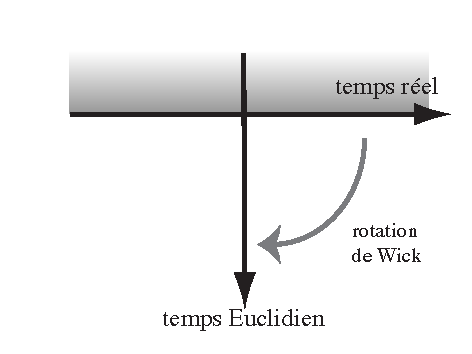
\includegraphics[width=6.cm]{Temps-imaginaire.pdf}
\caption{Real time $t$ and imaginary (Euclidean) time $\tau=\imath t$: Wick rotation }
\label{mqtf6}
\end{center}
\end{figure}

Consider now the case where $t$  is purely imaginary
\begin{equation}
\label{mqtim3}
t=-\imath\,\tau\quad,\quad\tau>0\quad\text{real}
\qquad\,\quad
U(-\imath\tau)=\exp\left(-{\tau\over\hbar} H\right)
\end{equation}
The evolution operator has the same form than the density matrix for the system in a Gibbs state at temperature $T$
\begin{equation}
\label{rhovsU}
\rho_\beta\ =\ {1\over Z(\beta)}\,  U(-\imath\tau)
\qquad,\quad \beta={1\over k_{\mathrm{B}}\,T}={\tau\over\hbar}={\imath}\ {t\over\hbar}
\end{equation}
For relativistic quantum field theories, time became an ``Euclidean coordinate'' $\tau=x^0$, and Minkowski space time becomes Euclidean space.
\index{Euclidean space}\index{Minkowski space}
There is deep analogy
\begin{center}
imaginary time $=$\ finite temperature
\end{center}
This analogy has numerous applications. It is at the basis of many applications of quantum field theory to statistical physics (Euclidean Field Theory).
Reciprocally, statistical physics methods have found applications in quantum physics and high energy physics (lattice gauge theories).
 Considering quantum theory for imaginary time is also very useful in high energy physics, in quantum gravity. Finally this relation between Gibbs (KMS) states and the unitary evolution operator extends to a more general relation between states and automorphisms of some operator algebras (Tomita-Takesaki theory), that we shall discuss (very superficially) in the next chapter.

\section{Path and functional integrals formulations}

\subsection{Path integrals}
\index{Path integral}\index{Feynman}
It is known since Feynman that a very useful, if not always rigorous, way to represent matrix elements of the evolution operator of a quantum system (transition amplitudes, or ``propagators'') is  provided by path integrals (for non-relativistic systems with a few degrees of freedom) and functional integrals (for relativistic or non relativistic systems with continuous degrees of freedoms, i.e. fields).

Standard references on path integral methods on quantum mechanics and quantum field theory are the original book by Feynman \& Hibbs \cite{FeynmanHibbs}, and the books by J. Zinn-Justin \cite{ZinnJustin-book}, \cite{Zinn-Justin:2010fk}.

For a single particle in an external potential this probability amplitude $K$ for propagation from $q_i$ at time $t_i$ to $q_f$ at time $t_f$\
\begin{equation}
\label{ }
\langle q_f|U(t_f-t_i)|q_i\rangle= \langle q_f,t_f|q_i,t_i\rangle\qquad U(t)=\exp\left({t\over i \hbar} H\right)
\end{equation}
(the first notation refers to the Schr�dinger picture, the second one to the Heisenberg picture) 
\index{Schr�dinger picture}\index{Heisenberg picture}
can be written as a sum of histories $q(t)$
\begin{equation}
\label{ }
\int_{q(t_i)=q_I,\ q(t_f)=
q_f}  \mathcal{D}[q]\ \exp\left({i\over \hbar} S[q]\right)
\end{equation}
where $S[q]$ is the classical action.
\index{Action}


\begin{figure}[h!]
\begin{center}
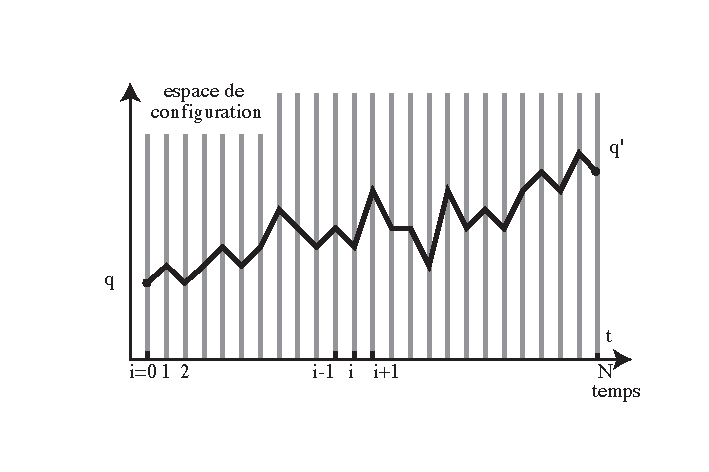
\includegraphics[width=4in]{trajectoires-discret.pdf}
\caption{Path integral: time discretization}
\label{ }
\end{center}
\end{figure}

The precise derivation of this formula, as well as its proper mathematical definition, is obtained by decomposing the evolution of the system in a large number $N$ of evolutions during  elementary time step $\Delta t=\epsilon=t/N$, at arbitrary intermediate positions $q(t_n=n\epsilon)$, $n\in\{1,\cdots ,N-1\}$, using the superposition principle.
One then uses the explicit formula for the propagation kernel at small time (the potential $V(q)$ may be considered as constant locally)
\begin{equation}
\label{ }
K(q_f,\epsilon, q_i,0)\simeq \left({2 i \pi \hbar\epsilon\over m}\right)^{-1/2}\ \exp\left({i\over \hbar}\left({m\over 2} {(q_f-q_i)^2\over \epsilon}-\epsilon V\left({q_f+q_i\over 2}\right)\right)\right) 
\end{equation}
and one then takes the continuous time limit $\epsilon\to 0$.
The precise definition of the measure over histories or paths  is (from the prefactor)
\begin{equation}
\label{ }
\mathcal{D}[q]=\prod_{n=1}^{N-1} \left(dq(t_n)\left({2 i \pi \hbar \epsilon\over m}\right)^{-1/2}\right)
\end{equation}

\index{Lagrangian}\index{Hamiltonian}
The  ``Lagrangian'' path integral has a ``Hamiltonian'' version (path integral in phase space)
\begin{equation}
\label{ }
\int_{q(t_i)=q_I,\ q(t_f)=
q_f}  \mathcal{D}[q,p]\ \exp\left({i\over \hbar} \int dt\left(p \dot q -H(q,p))\right)\right)
\end{equation}
But one must be very careful on the definition of this path integral (discretization and continuum time limit) and on the measure in order to obtain a consistent quantum theory. 

\subsection{Field theories, functional integrals}

\index{Functional integral}
\index{Quantum field theory}
Path integral representations extend to the case of relativistic quantum field theories. For instance for the scalar field, whose classical action (giving the Klein-Gordon equation) is
\index{Scalar field}\index{Klein-Gordon equation}
\begin{equation}
\label{ }
S[\phi]=\int dt \int d^3\vec x\ {1\over 2} \left(\left({\partial\phi\over\partial t}\right)^2- \left({\partial\phi\over\partial \vec x}\right)^2 - m^2 \phi^2\right)
=\int d^4x {1\over 2} \left(-\partial^\mu\phi\, \partial_\mu \phi - m^2 \phi^2\right)  
\end{equation}
a path integral involves an integral over field configurations over space-time of the form
$$\int \mathcal{D}[\phi)\ \emath^{{\imath\over\hbar} S[\phi]}$$
and is usually denoted a functional integral.

\index{Time ordered product}
More precisely, the vacuum expectation value of time ordered product of local field operators $\boldsymbol{\phi}$  in this quantized  field theory can be expressed as a functional integral
\begin{equation}
\label{ }
\langle\Omega|T \boldsymbol{\phi}(x_1)\cdots \boldsymbol{\phi}(x_N)|\Omega\rangle={1\over Z}
\int \mathcal{D}[\phi)\ \emath^{{\imath\over\hbar} S[\phi]}\phi(x_1)\cdots\phi(x_N)
\end{equation}
with $Z$ the partition function or vacuum amplitude
\begin{equation}
\label{ }
{Z}=
\int \mathcal{D}[\phi)\ \emath^{{\imath\over\hbar} S[\phi]}
\end{equation}
The factor $Z$ means that the functional integral is normalized so that the vacuum to vacuum amplitude is $$\langle\Omega|\Omega\rangle=1$$

The path integral and functional integral formulations are invaluable tools to formulate many quantum systems and quantum field theories, and perform calculations. 
They give a very simple and intuitive picture of the semiclassical regimes. It explains why the laws of classical physics can be formulated via variational principles, since classical trajectories are just the stationary phase trajectories (saddle points) dominating the sum over trajectories in the classical limit $\hbar\to 0$.
In many cases it allows to treat and visualize quantum interference effects when a few semi-classical trajectories dominates (for instance for trace formulas).

Functional integral methods are also very important conceptually for quantum field theory: from the renormalization of QED to the quantization and proof of renormalisability of non abelian gauge theories, the treatment of topological effects and anomalies in QFT, the formulation of the Wilsonian renormalization group, the applications of QFT methods to statistical mechanics, etc.
They thus provides a very useful way to quantize a theory, at least in semiclassical regime where one expect that the quantum theory is not too strongly coupled and quantum correlations and interference effects can be kept under control.

I will not elaborate further here. When discussing the quantum formalism, one should keep in mind that the path and functional integrals represent a very useful and powerful (if usually not mathematically rigorous) way to visualize, manipulate and compute transition amplitudes, i.e. matrix elements of operators. They  rather represent an application of the standard canonical formalism, allowing to construct the Hilbert space (or part of it) and the matrix elements of operators of a quantum theory out of a classical theory via a quick and efficient recipe.


{
\section{Quantum mechanics and reversibility}
}
\label{S:reversibility}
\index{Reversibility}
\index{Irreversibility}
\subsection{Is quantum mechanics reversible or irreversible?}
An important property of quantum  (as well as classical) physics is reversibility: 
the general formulation of the physical laws is the same under time reversal. 
This  is often stated as: 
\index{Time reversal}\index{Time arrow}
\begin{center}
``There is no microscopic time arrow.''
\end{center}
This does not mean that the fundamental interactions (the specific physical laws that govern our universe) are invariant under time reversal.
It is known that (assuming unitarity, locality and Lorentz invariance) they are invariant only under CPT, the product of charge conjugation, parity and time reversal. This reversibility statement means that the dynamics, viewed forward in time (press key \fbox{${\RHD}$} ), of any given state of a system is similar to the dynamics, viewed backward in time (press key \fbox{$\LHD$} ), of some other state.

This reversibility statement is of course also different from the macroscopic irreversibility that we experience in everyday life (expansion of the universe, second principle of Thermodynamics, quantum measurement, 
Parkinson's laws \cite{Parkinson1955}
, etc.).
\index{Second principle of thermodynamics}
\index{Parkinson's law}
\index{Measurement}

In classical mechanics reversibility is an obvious consequence of the Hamiltonian formulation. In quantum mechanics things are more subtle. Indeed if the evolution of a ``closed system'' (with no interaction with its environment or some observer) is unitary and reversible (and in particular possible quantum correlations between the system and its ``outside'' are kept untouched), quantum measurements are irreversible processes.
However it is known since a long time that microscopic reversibility is not really in contradiction with this irreversibility.
See for instance the '64 paper by Aharonov, Bergmann \& Lebowitz \cite{Aharonov1964}.
Since this will be very important in these following lectures, especially in the presentation of the quantum logic formalism, let us discuss it on a simple, but basic example, with the usual suspects involved in quantum measurements.

\subsection{Reversibility of quantum probabilities}
\label{ssRevQP}
We consider two observers, Alice and Bob. 
Each of them can  measure a different observable (respectively $A$ and $B$) on a given quantum system $\mathcal{S}$ (for simplicity $\mathcal{S}$ can be in a finite number of states, i.e. its Hilbert space is finite dimensional). We take these observations to be perfect (non demolition) test measurements, i.e. yes/no measurements, represented by some selfadjoint projectors $\mathbf{P}_A$ and $\mathbf{P}_B$ such that $\mathbf{P}_A^2=\mathbf{P}_A$ and $\mathbf{P}_B^2=\mathbf{P}_B$, but not necessarily commuting.
The eigenvalues of these operators are $1$ and $0$, corresponding to the two possible outcomes $1$ and $0$ (or $\TRUE$ and $\FALSE$ ) of the  measurements of the observables $A$ and of the observable $B$. 
\index{Observable}\index{Eigenvalue}\index{Eigenvector}




Let us consider now the two following protocols.

\paragraph{Protocol 1:}

\index{Alice}\index{Bob}\index{Measurement}
Alice gets the system $\mathcal{S}$ (in a state  she knows nothing about). She measures $A$ and if she finds $\TRUE$, then she send the system to Bob, who measures $B$. What is the plausibility
\footnote{In a Bayesian sense. 
}
 for Alice that Bob will find that $B$ is $\TRUE$? Let us call this the conditional probability for $B$ to be found true, $A$ being known to be true, and denote it $P(B{\,\mapsfrom\hskip -2.ex\vert\hskip 1.ex} A)$.
The arrow $\mapsfrom$ denotes the causal ordering between the measurement of $A$ (by Alice) and of $B$ (by Bob).
\index{Conditional probabilities}
\index{Causal ordering}
\index{Bayesian probabilities}

\begin{figure}[h]
\begin{center}
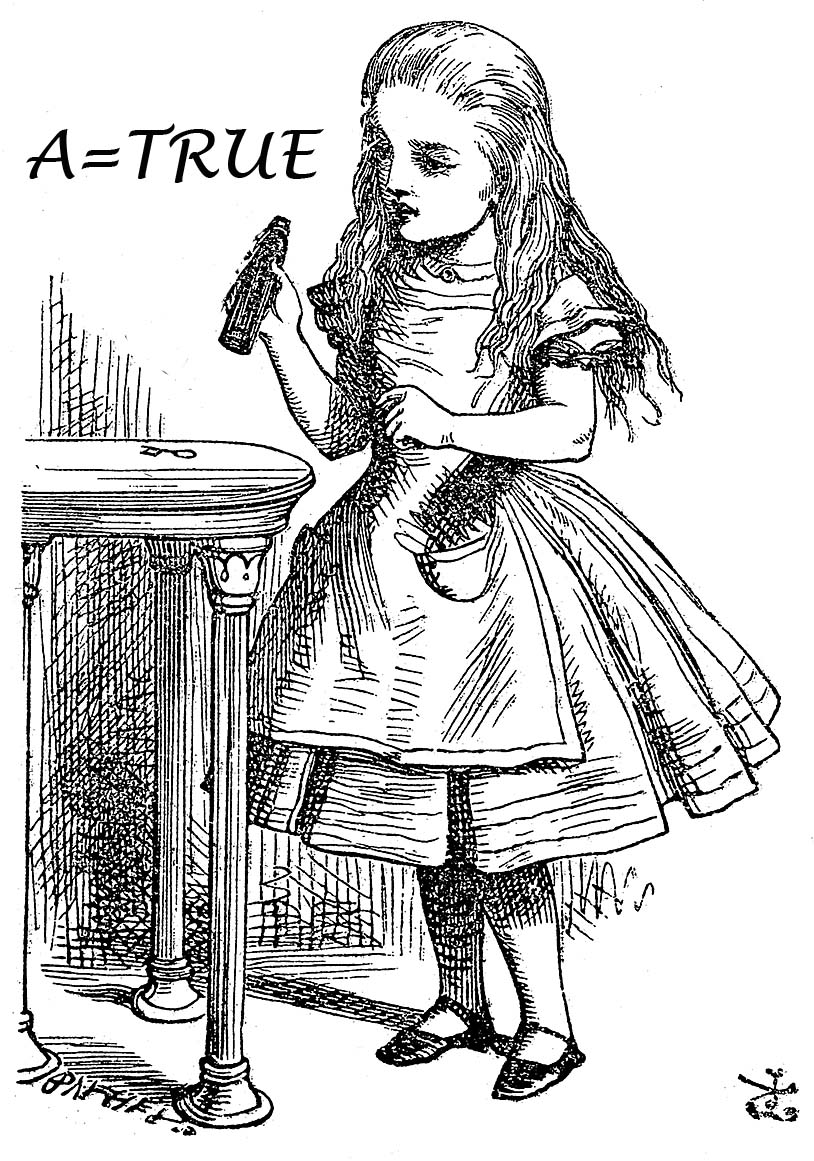
\includegraphics[width=2.in]{Alice-1.jpg}\qquad
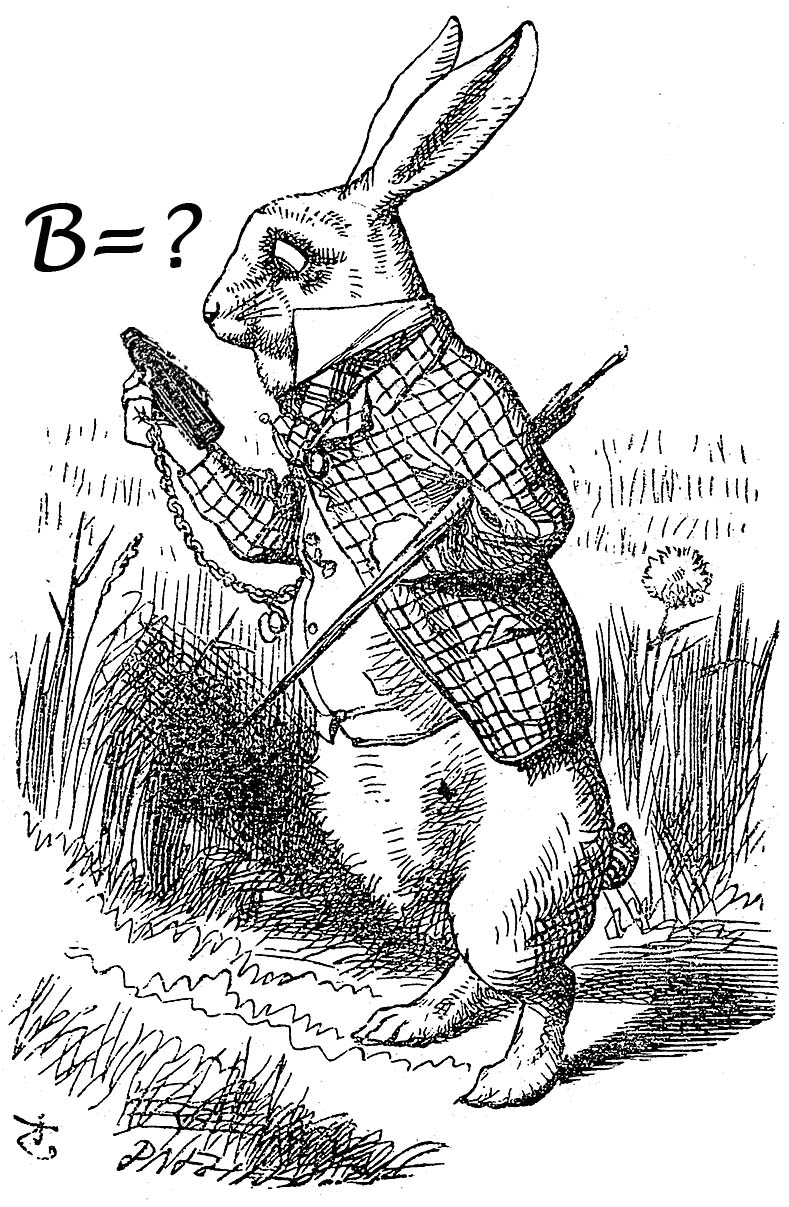
\includegraphics[width=2.in]{Bob-1.jpg}
\caption{Protocol 1: Alice wants to guess what Bob will measure. This defines the conditional probability  $ P(B{\,\mapsfrom\hskip -2.ex\vert\hskip 1.ex} A)$.}
\label{ }
\end{center}
\end{figure}

\paragraph{Protocol 2:}


  Alice gets the system $\ {S}$ from Bob, and knows nothing else about $\mathcal{S}$. Bob tells her that he has measured $B$, but does not tell her the result of his measurement, nor how the system was prepared before he performed the measurement (he may know nothing about it, he just measured $B$). Then Alice measures $A$ and (if) she finds $\TRUE$ she asks herself the following question: what is the plausibility 
(for her, Alice) that Bob had found that $B$ was $\TRUE$? 
\footnote{This question makes sense if for instance, Alice has made a bet with Bob. Again, and especially for this protocol, the probability has to be taken in a Bayesian sense.}
Let us call this the conditional probability for $B$ to have been found true, $A$ being known to be true, and denote it by 
$P(B{\,\mapsto\hskip -2.3ex\vert\hskip 1.ex} A)$.
The arrow $\mapsto$ denotes the causal ordering between the measurement of $A$ (by Alice) and of $B$ (by Bob).

  \begin{figure}[h!]
\label{ }
\begin{center}
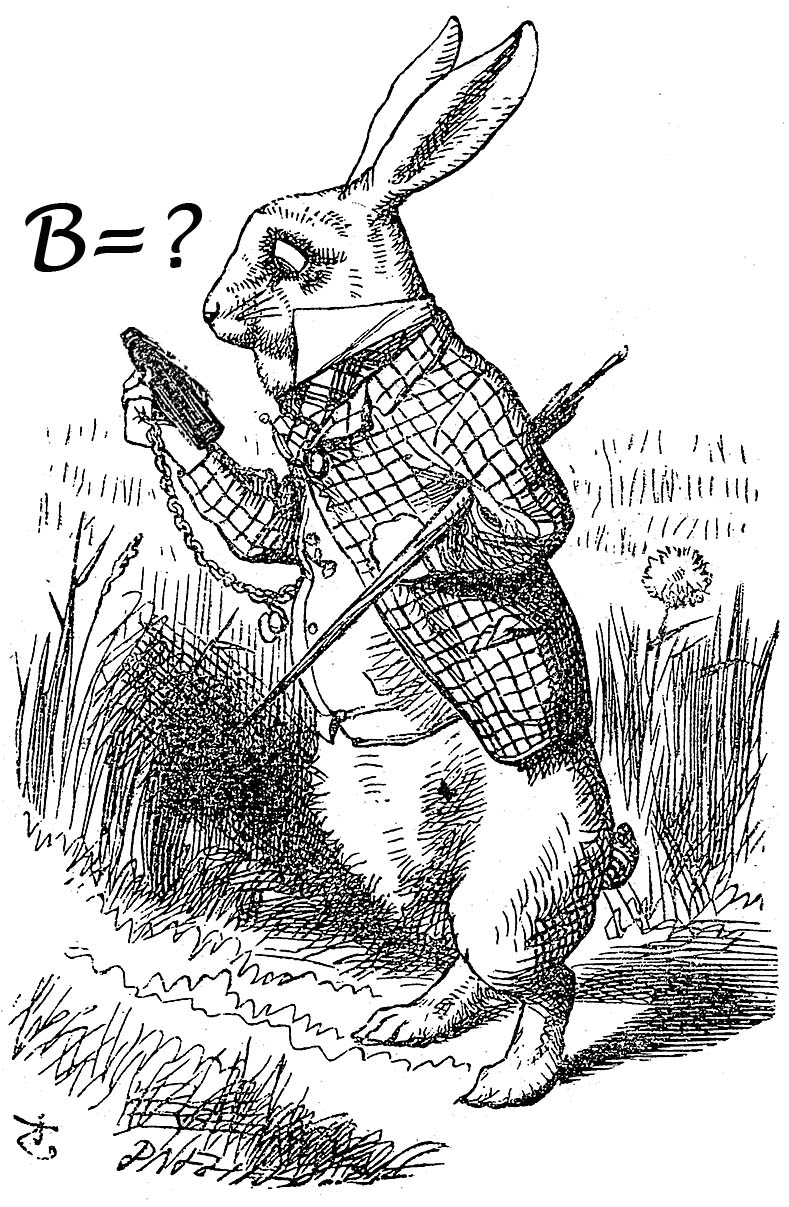
\includegraphics[width=2.in]{Bob-1.jpg}\qquad
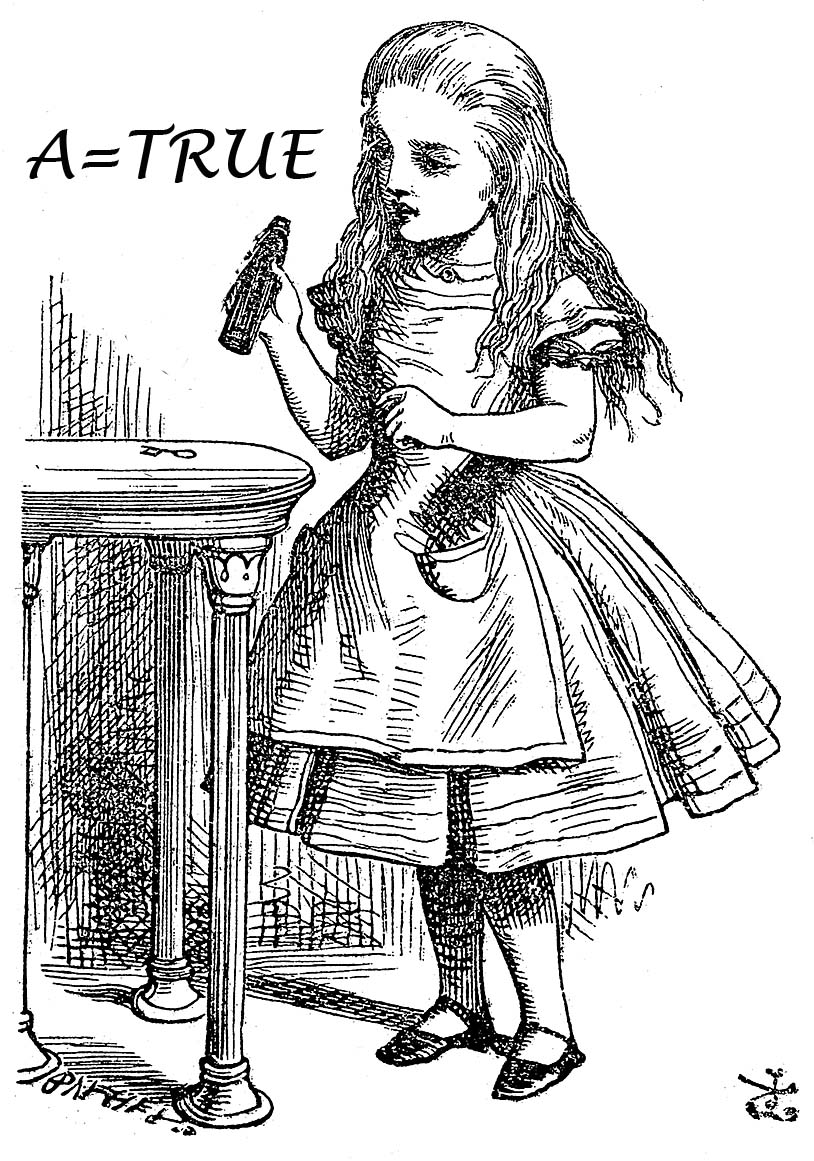
\includegraphics[width=2.in]{Alice-1.jpg}\nonumber\\
\caption{Protocol 2: Alice wants to guess what Bob has measured. This defines the conditional probability  \quad $P(B{\,\mapsto\hskip -2.ex\vert\hskip 1.ex} A)$.}
\end{center}
\end{figure}


\iffalse
\begin{enumerate}
  \item Alice gets the system $\mathcal{S}$ (in a state  she knows nothing about), she measures $A$ and if she finds $\TRUE$, then she sends the system to Bob, who measures $B$. What is the plausibility\footnote{In a Bayesian sense. I refer to \cite{} for a discussion of Bayesian probabilities.} for Alice that Bob will find that $B$ is $\TRUE$? Let us call this the conditional probability for $B$ to be found true, $A$ being known to be true, and denote it $P(B{\,\mapsfrom\hskip -2.ex\vert\hskip 1.ex} A)$.
The arrow $\mapsfrom$ denotes the causal ordering between the measurement of $A$ (by Alice) and of $B$ (by Bob).

\begin{align}
\label{ }
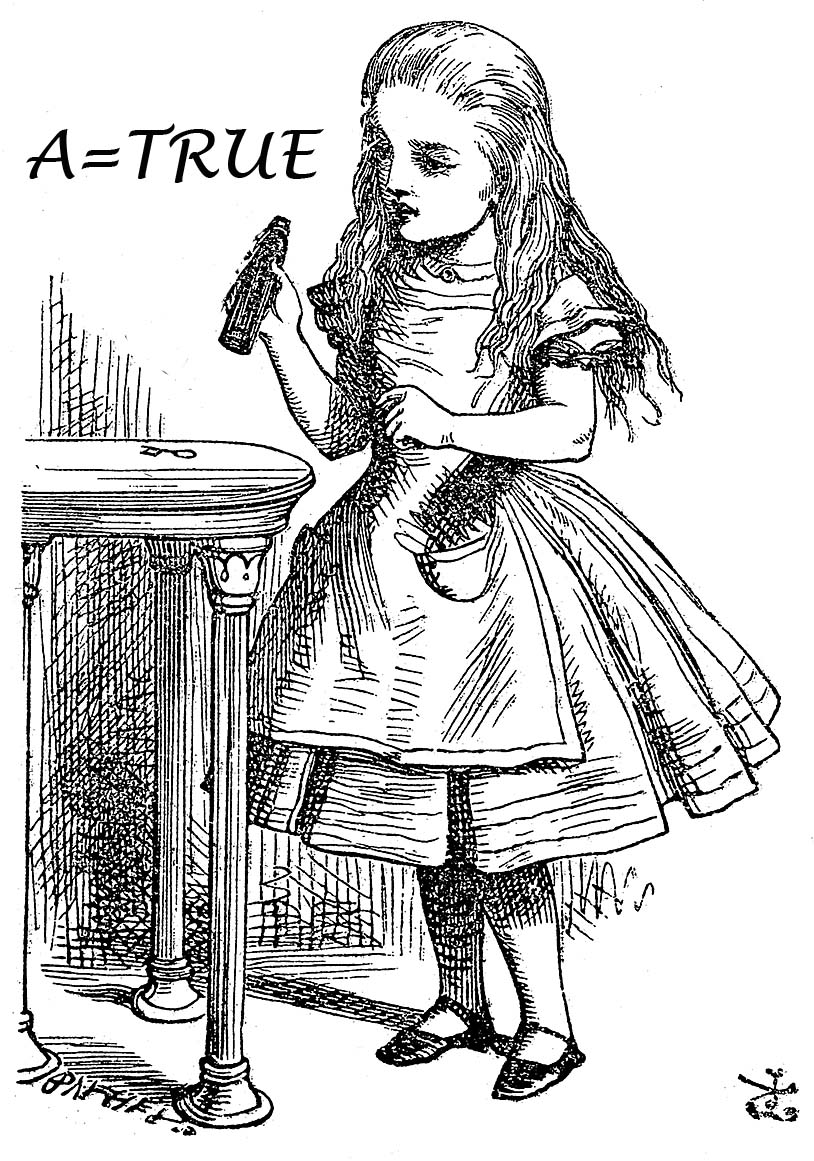
\includegraphics[width=2.in]{Alice-1.jpg}\qquad
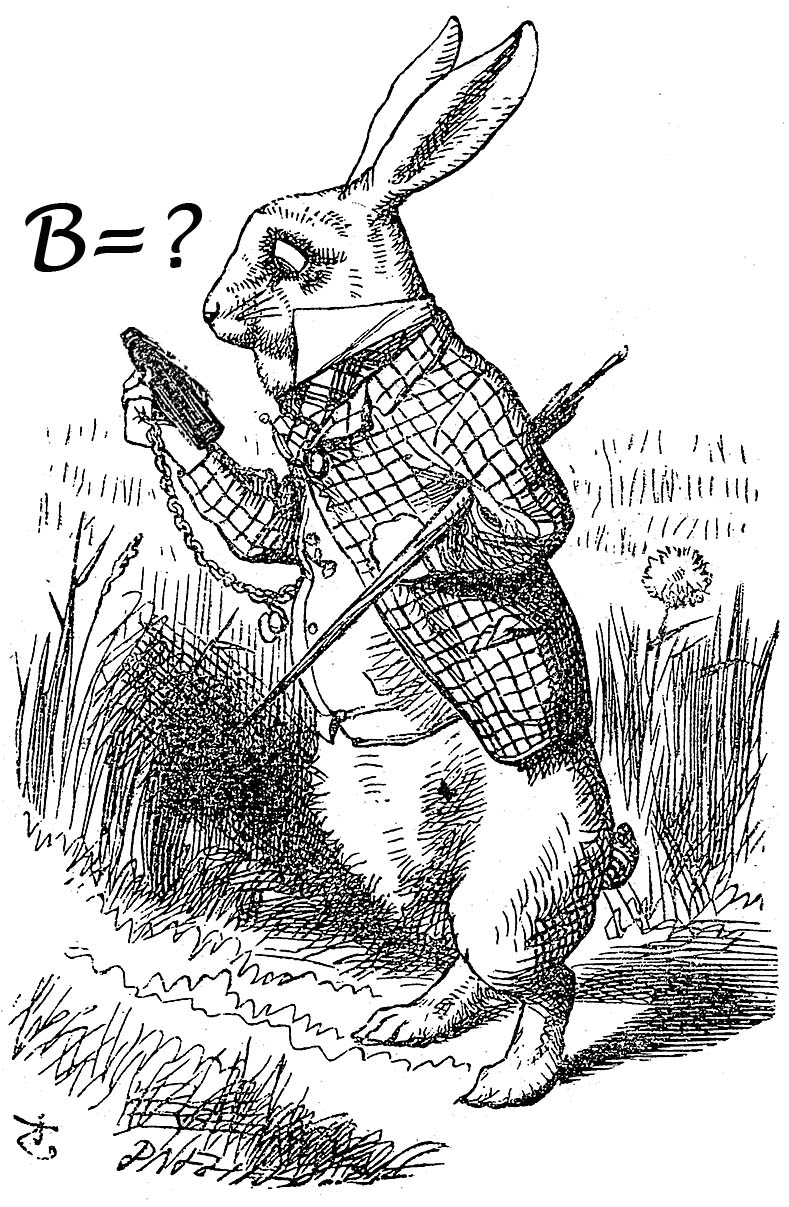
\includegraphics[width=2.in]{Bob-1.jpg}\nonumber\\
\text{Protocol 1: Alice wants to guess what Bob will measure \quad} P(B{\,\mapsfrom\hskip -2.ex\vert\hskip 1.ex} A)\   .
\end{align}

    \item Alice gets the system $\mathcal{S}$ from Bob, and knows nothing else about $\mathcal{S}$. Bob tells her that he has measured $B$, but does not tell her the result of his measurement, nor how the system was prepared before he performed the measurement (he may know nothing about it, he just measured $B$). Then Alice measures $A$ and (if) she finds $\TRUE$ she asks herself the following question: what is the plausibility %\footnote{again, and especially for this protocol, in a Bayesian sense.} 
(for her, Alice) that Bob had found that $B$ was $\TRUE$? 
\footnote{This question makes sense if for instance, Alice has made a bet with Bob. Again, and especially for this protocol, the probability has to be taken in a Bayesian sense.}
Let us call this the conditional probability for $B$ to have been found true, $A$ being known to be true, and denote it by 
$P(B{\,\mapsto\hskip -2.3ex\vert\hskip 1.ex} A)$.
The arrow $\mapsto$ denotes the causal ordering between the measurement of $A$ (by Alice) and of $B$ (by Bob).

\begin{align}
\label{ }
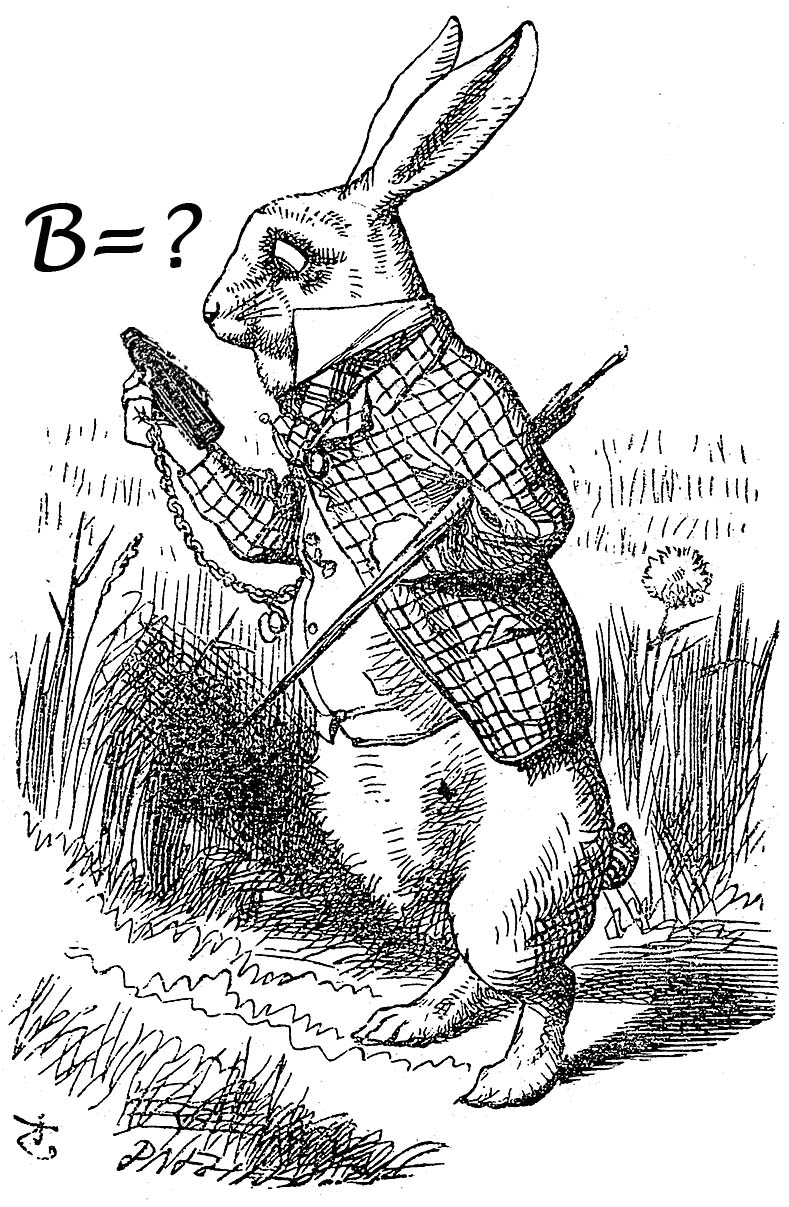
\includegraphics[width=2.in]{Bob-1.jpg}\qquad
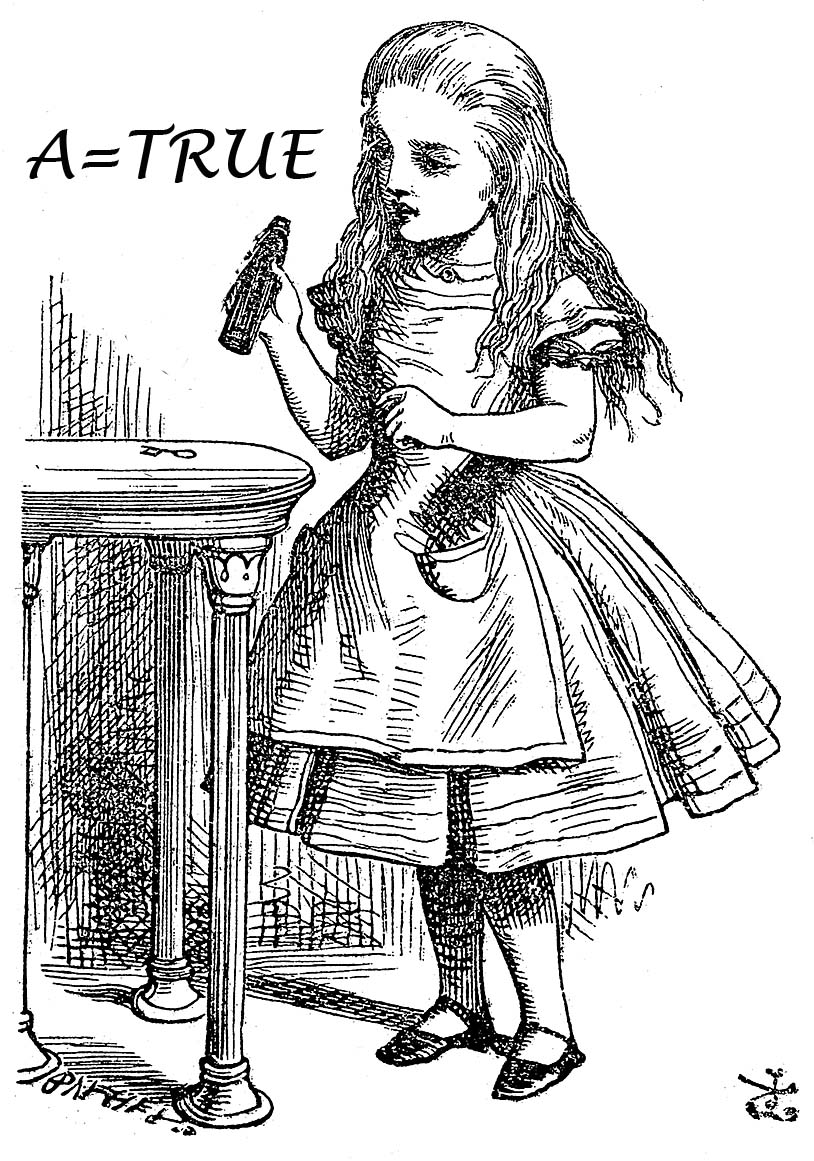
\includegraphics[width=2.in]{Alice-1.jpg}\nonumber\\
\text{Protocol 2: Alice wants to guess what Bob has measured \quad}P(B{\,\mapsto\hskip -2.ex\vert\hskip 1.ex} A)\   .
\end{align}

\end{enumerate}
\fi
%%%%%%%%%%%%%

If $\mathcal{S}$ was a classical system, and the mesurements  were classical measurements which do not change the state of $\mathcal{S}$,  then the two protocols are equivalent and  the two quantities  equal  the standard conditional probability (Bayes formula)
$$\mathcal{S}\ \text{classical system}\,:  \ \ P(B{\,\mapsfrom\hskip -2.ex\vert\hskip 1.ex} A) =P(B{\,\mapsto\hskip -2.3ex\vert\hskip 1.ex} A)=P(B|A)=P(B\cap A)/P(A)\ .$$
\index{Bayes formula}

In the quantum case, at a purely logical level, knowing only that the measurement process may perturb the system $\mathcal{S}$, $P(B{\,\mapsfrom\hskip -2.ex\vert\hskip 1.ex} A)$ and $P(B{\,\mapsto\hskip -2.3ex\vert\hskip 1.ex} A)$ may be different. 
A crucial and remarkable property of quantum mechanics is that they are still equal. Indeed in the first protocol $P(B{\,\mapsfrom\hskip -2.ex\vert\hskip 1.ex} A)$ is given by the Born rule; if Alice finds that $A$ is $\TRUE$ and knows nothing more, her best bet is that the state of $\mathcal{S} 
$ is given by the density matrix 
$$\rho_A=\mathbf{P}_A/\mathrm{Tr}(\mathbf{P}_A)$$
Therefore the probability for Bob to find that $B$ is $\TRUE$ is 
$$P(B{\,\mapsfrom\hskip -2.ex\vert\hskip 1.ex} A)=\tr(\rho_A\mathbf{P}_B) .$$


In the second protocol the best guess for Alice is to assume that before Bob measures $B$ the state of the system is given by the equidistributed density matrix $\rho_{\mathbf{1}}=\mathbf{1}/\tr(\mathbf{1})$.  
In this case the probability that Bob finds that $B$ is $\TRUE$, then that Alice finds that $A$ is $\TRUE$, is 
$$p_1=\tr(\mathbf{P}_B)/\tr(\mathbf{1})\times \tr(\rho_B\mathbf{P}_A)
\quad\text{ with}\quad
\rho_B=\mathbf{P}_B/\mathrm{Tr}(\mathbf{P}_B).$$
Similarily the probability that  Bob finds that $B$ is $\FALSE$, then that Alice finds that $A$ is $\TRUE$ is 
$$p_2=\tr(\mathbf{1}-\mathbf{P}_{B})/\tr(\mathbf{1})\times \tr(\rho_{\overline B}\mathbf{P}_A)=(\tr(\mathbf{P}_A)-\tr(\mathbf{P}_A\mathbf{P}_B))/\tr(\mathbf{1})$$
 where $\rho_{\overline B}=(\mathbf{1}-\mathbf{P}_B)/\tr(\mathbf{1}-\mathbf{P}_B)$. 
 The total probability is then 
 $$ P(B{\,\mapsto\hskip -2.3ex\vert\hskip 1.ex} A)= p_1+p_2 = \tr(\rho_A\mathbf{P}_B) .$$
 
Therefore, even if $A$ and $B$ are not compatible, i.e. if  $\mathbf{P}_A$ and $\mathbf{P}_B$ do not commute, we obtain in  both case the standard result for quantum conditional probabilities
\begin{equation}
\label{ }
\mathcal{S}\ \text{quantum system}\, :\ \ 
P(B{\,\mapsfrom\hskip -2.ex\vert\hskip 1.ex} A)=P(B{\,\mapsto\hskip -2.3ex\vert\hskip 1.ex} A)=\mathrm{Tr}[\mathbf{P}_A \mathbf{P}_B]/ \mathrm{Tr}[\mathbf{P}_A]
\end{equation}

This reversibility property (that I denote here causal reversibility, in order not to confuse it with time reversal invariance) is very important, as we shall see later.\index{Causal reversibility}

